\subsection{Physiological data}

The same sensors used for the first objective are used for the second objective. The expectations for all of the results is a difference between the “blind” sample and the “sight” sample. This subsection was divided in the same way as before:

\begin{itemize}
    \item \nameref{subsubsec:results_ecg_2};
    
        Two features are extracted from the ECG, heartrate (BPM) and heartrate variance (SDNN).
    
        Is expected that the heartrate increases at every “First” round and then a slight decrease in the next round. The heartrate variance is expected to decrease in the “First” round and a slight increase in the next round.    

    \item \nameref{subsubsec:results_gsr_temp_2};
    
        Is expected that the GSR average to increase at every “First” round and then a slight decrease in the next round.

\end{itemize}
\subsubsection{Electrocardiogram (ECG) data}
\label{subsubsec:results_ecg_2}

\paragraph{Analysis of the heartbeat frequency (BPM)}\mbox{}\\

Table \ref{tab:bpm_table_noBase} presents the average heart rate for both sighted and blind groups. The barplots are presented in Figure \ref{fig:barplot_ecg_bpm_4_scene_blind_sight}. Comparing the two groups, the audio method is associated with a slightly lower heartrate for blind people, but the opposite happens for sighted participants. Moreover, data from blind participants have large variance. This large variance can also be observed in the boxplot of Figures \ref{fig:boxplot_ecg_bpm_4_scene} and \ref{fig:boxplot_ecg_bpm_4_rounds}. 


\begin{table}[!htb]
\centering
\caption{ECG average BPM felled by the participants using the proposed methods [BPM].}
\label{tab:bpm_table_noBase}
\begin{tabular}{lllrrrrr}
\toprule
    &       &        &  Audio & \begin{tabular}[c]{@{}l@{}}Haptic\\ Belt\end{tabular} & \begin{tabular}[c]{@{}l@{}}Virtual\\ Cane\end{tabular} & Mixture \\
Part. & \begin{tabular}[c]{@{}l@{}}Visual\\ Condition\end{tabular} & Round &        &                                                       &                                                        &         \\
\midrule
001 & Sight & First &  71.23 &                                                 63.02 &                                                  64.85 &   58.77 \\
    &       & Return &  73.18 &                                                 61.18 &                                                  66.78 &   66.26 \\
001C & Blind & First &  60.71 &                                                 71.17 &                                                  59.07 &   68.24 \\
    &       & Return &  58.61 &                                                 66.22 &                                                  64.20 &   70.76 \\
002C & Blind & First &  38.67 &                                                 48.74 &                                                  46.89 &   52.23 \\
    &       & Return &  47.58 &                                                 58.97 &                                                  56.75 &   58.25 \\
003 & Sight & First &  63.47 &                                                 71.80 &                                                  70.90 &   72.76 \\
    &       & Return &  72.75 &                                                 71.23 &                                                  67.49 &   73.01 \\
003C & Blind & First &  69.89 &                                                 70.95 &                                                  69.41 &   66.94 \\
    &       & Return &  67.44 &                                                 69.68 &                                                  68.82 &   67.37 \\
004 & Sight & First &  66.85 &                                                 62.45 &                                                  65.94 &   67.86 \\
    &       & Return &  69.48 &                                                 65.65 &                                                  64.58 &   71.86 \\
004C & Blind & First &  73.55 &                                                 73.70 &                                                  71.94 &   74.03 \\
    &       & Return &  74.79 &                                                 74.02 &                                                  72.69 &   67.34 \\
005 & Sight & First &  71.34 &                                                 66.93 &                                                  66.46 &   67.06 \\
    &       & Return &  69.57 &                                                 65.97 &                                                  67.00 &   65.47 \\
\bottomrule
\end{tabular}
\end{table}



\begin{figure}[!htpb]
    \centering
    \begin{minipage}{\textwidth}
        \centering
        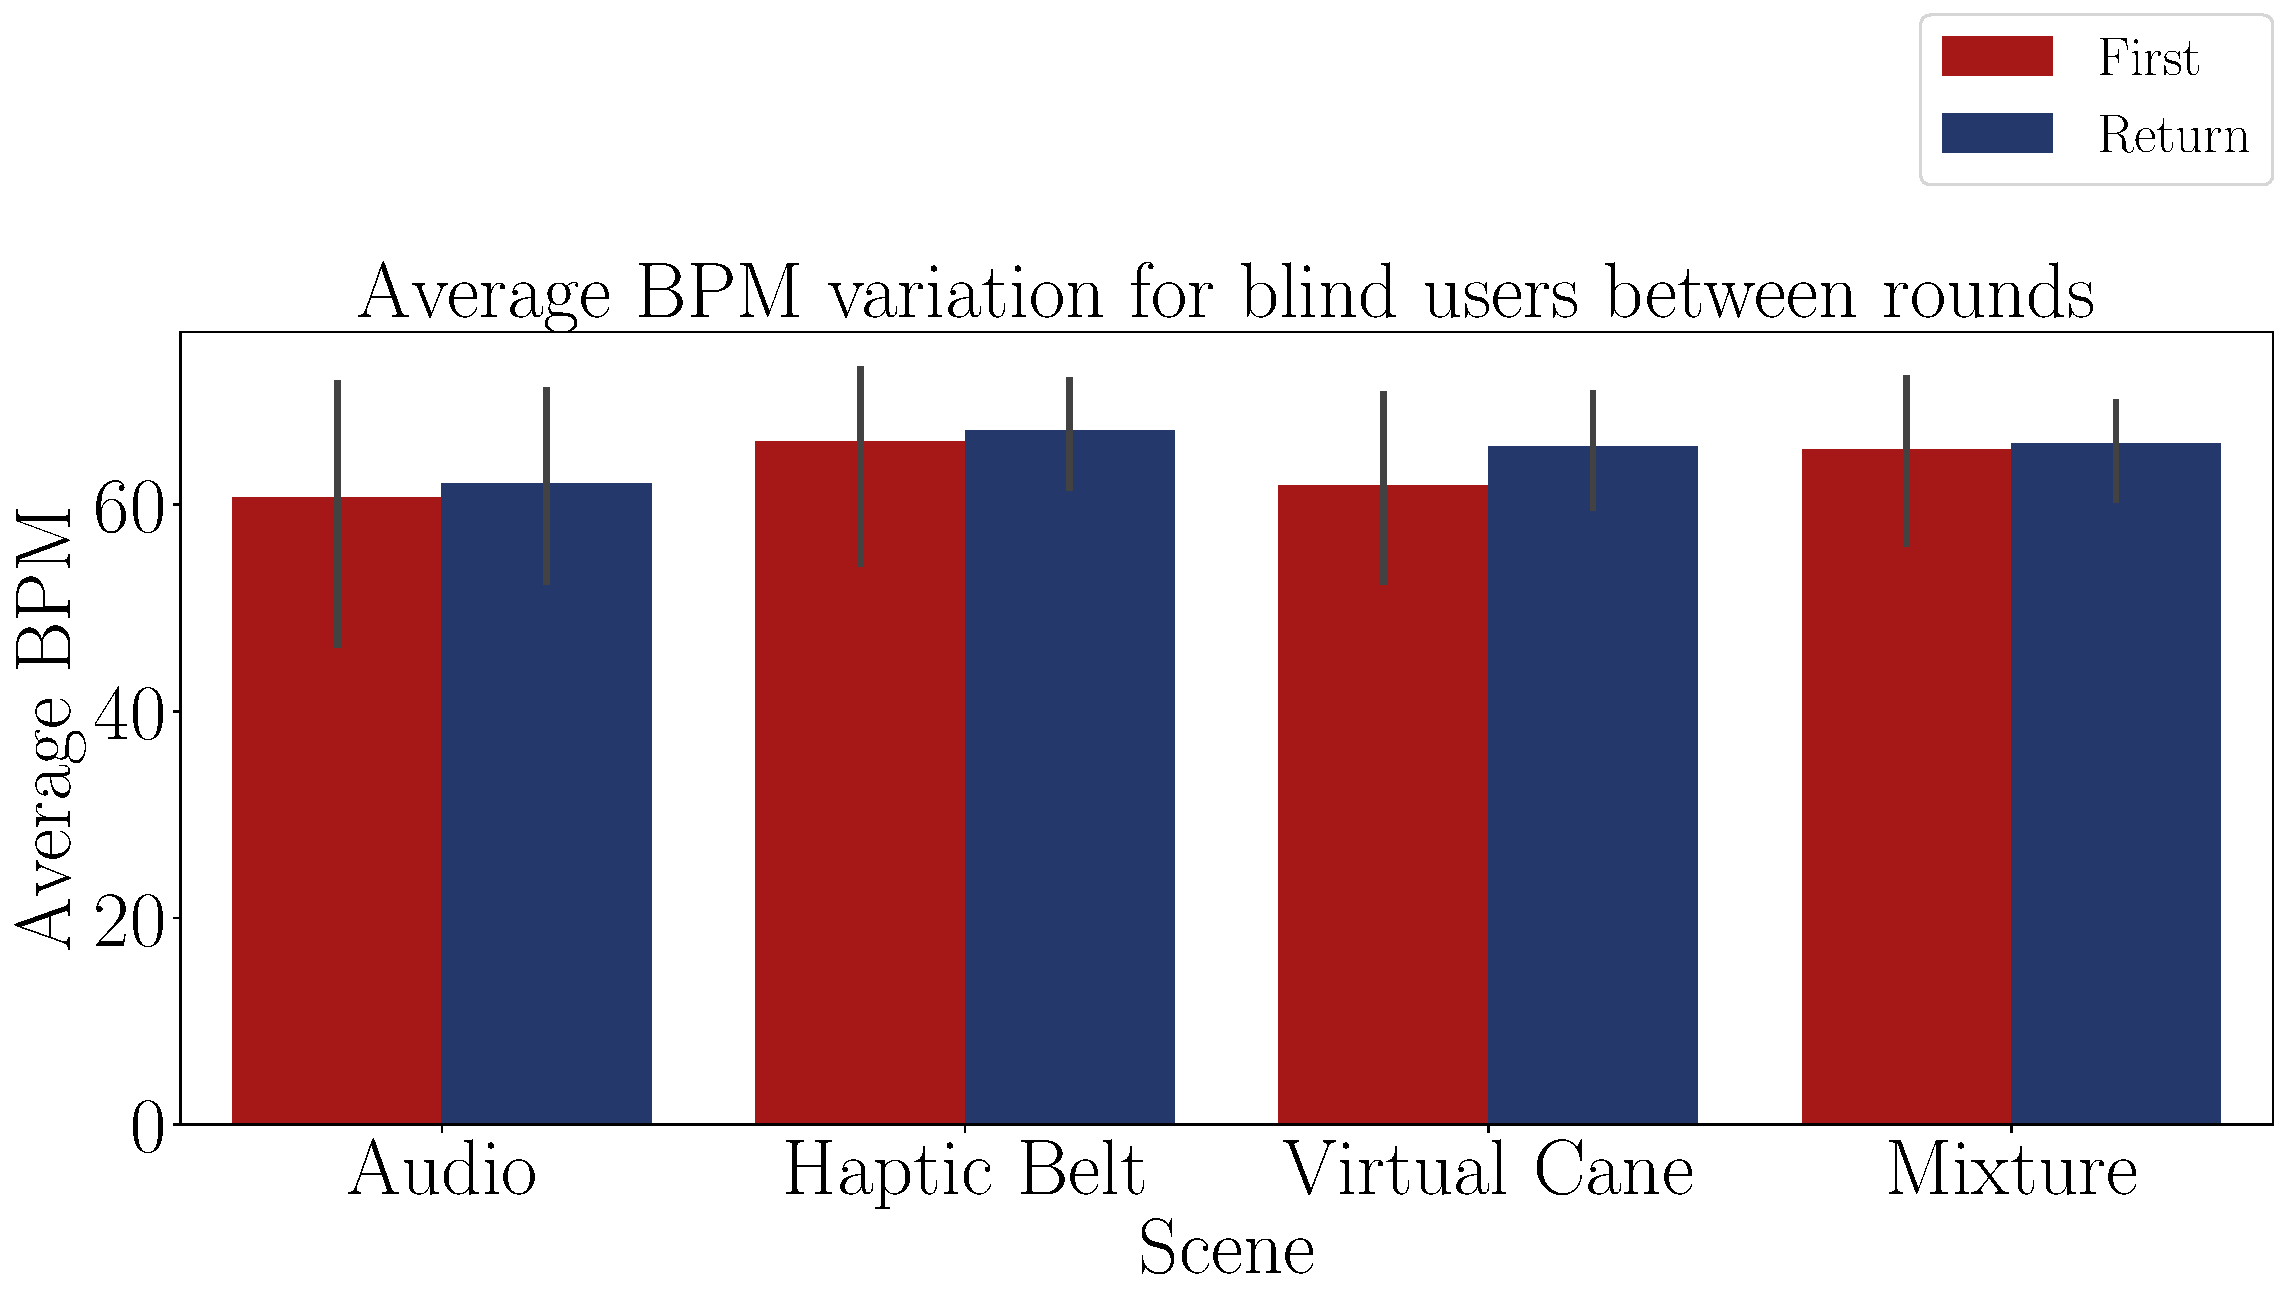
\includegraphics[width = 0.8\linewidth]{Resultados/ECG/Figuras/pdf/barplot_ecg_bpm_4_scene_blind.pdf}
        \subcaption{Blind participants.}
        \label{fig:barplot_ecg_bpm_4_scene_blind}
    \end{minipage}
    \begin{minipage}{\textwidth}
        \centering
        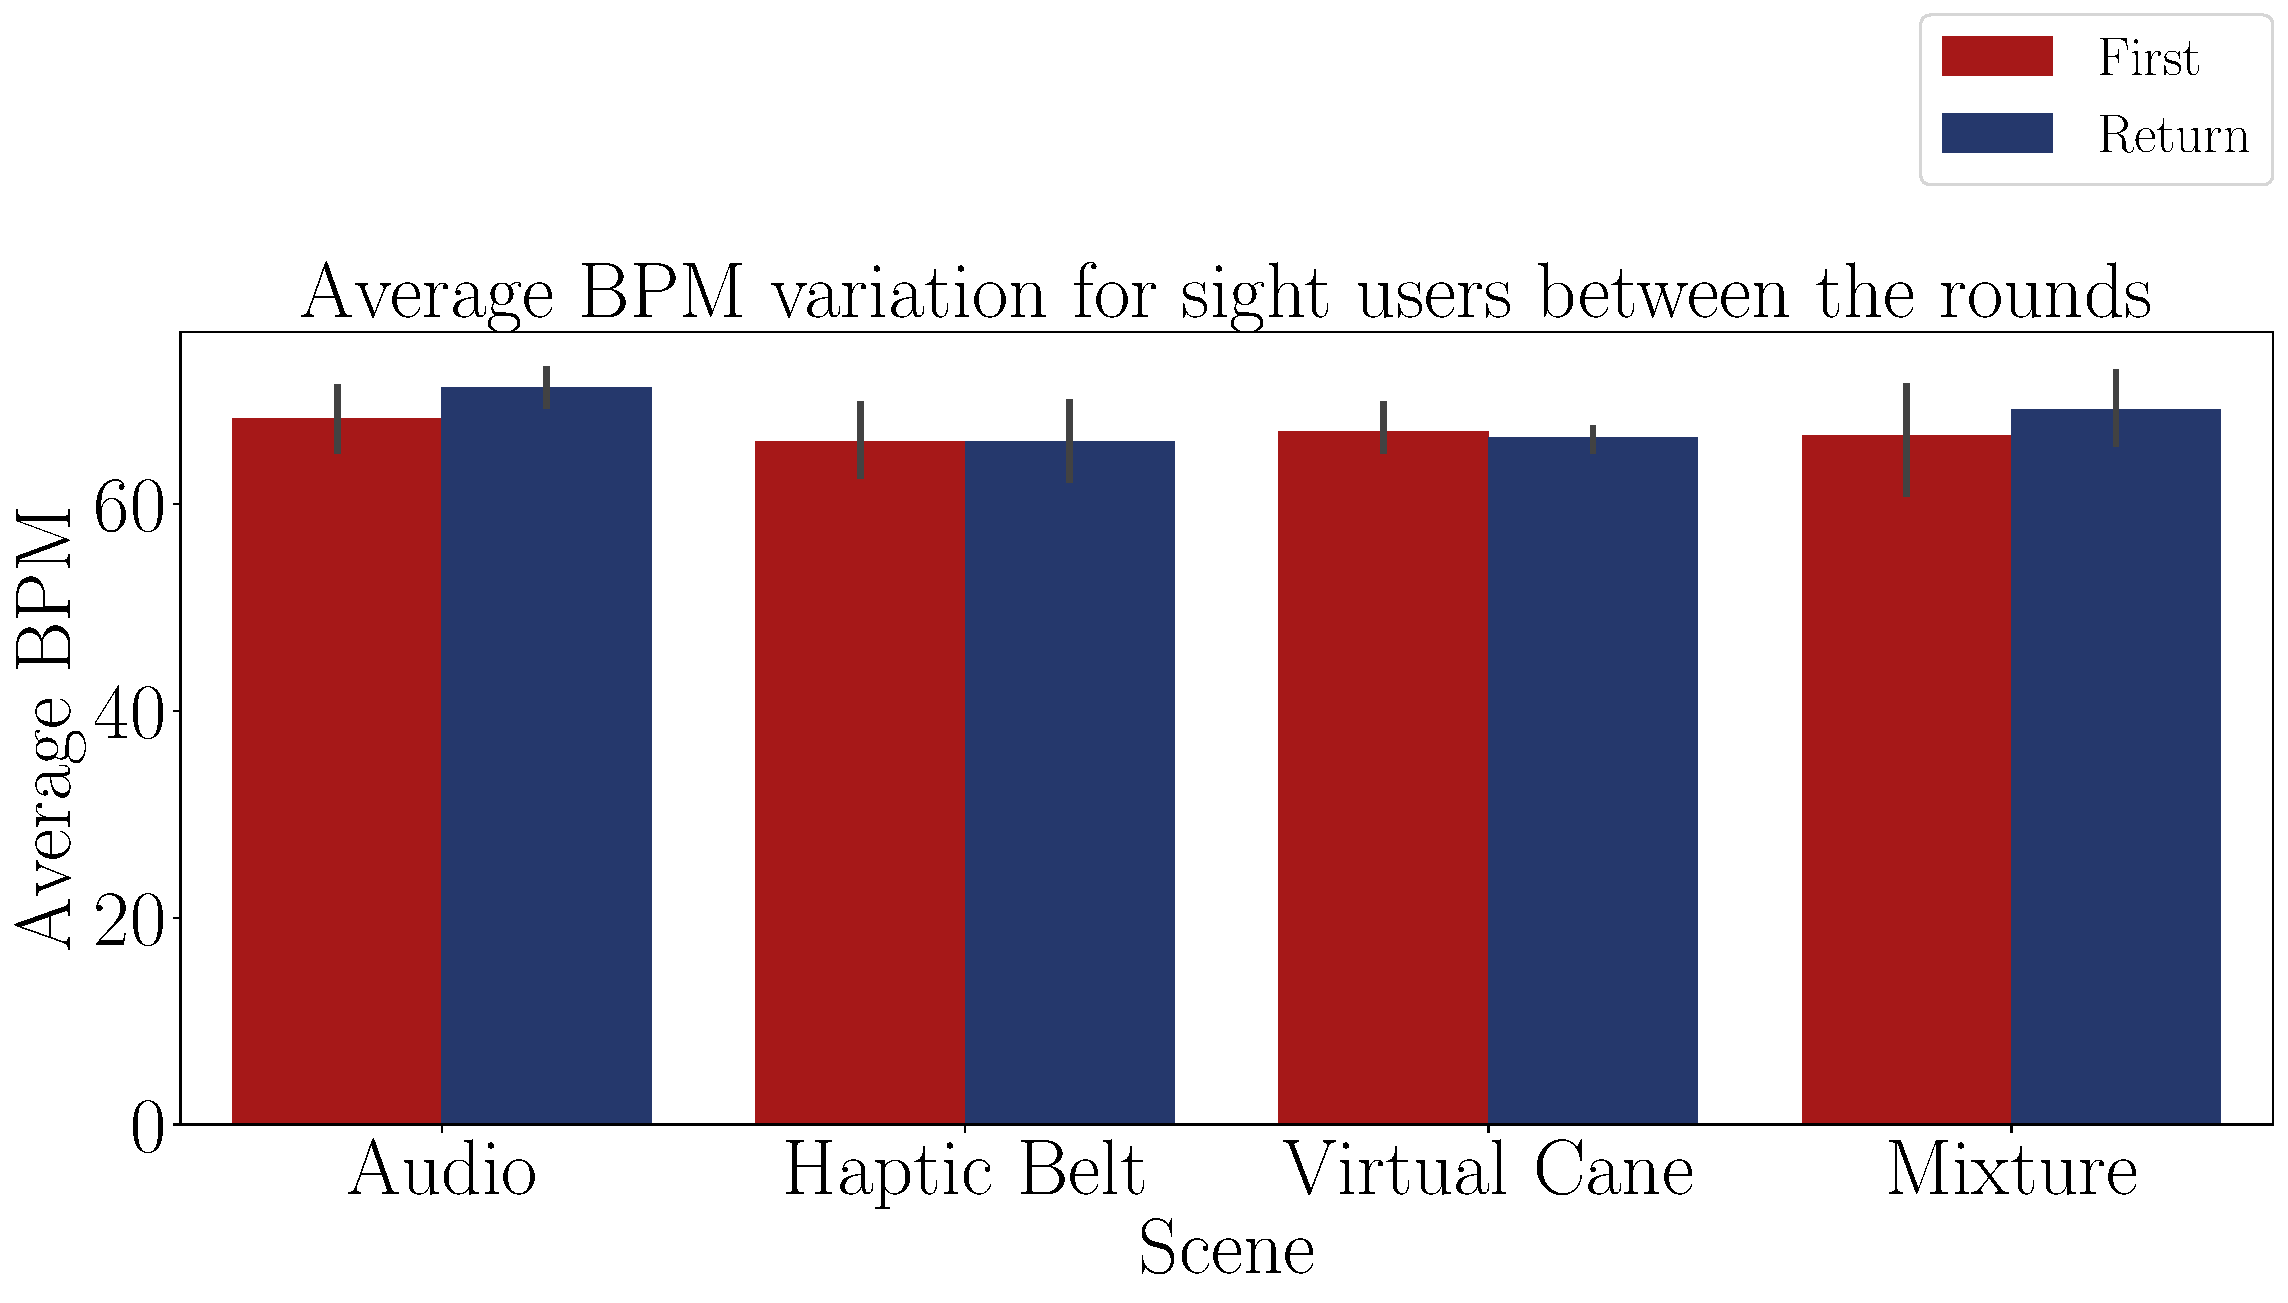
\includegraphics[width = 0.8\linewidth]{Resultados/ECG/Figuras/pdf/barplot_ecg_bpm_4_scene_sight.pdf}
        \subcaption{Sight participants.}
        \label{fig:barplot_ecg_bpm_4_scene_sight}
    \end{minipage}
    \caption{Barplot of the average BPM of the on each ethod and round.}
    \label{fig:barplot_ecg_bpm_4_scene_blind_sight}
\end{figure}
%\begin{figure}[!htpb]
%    \centering
%    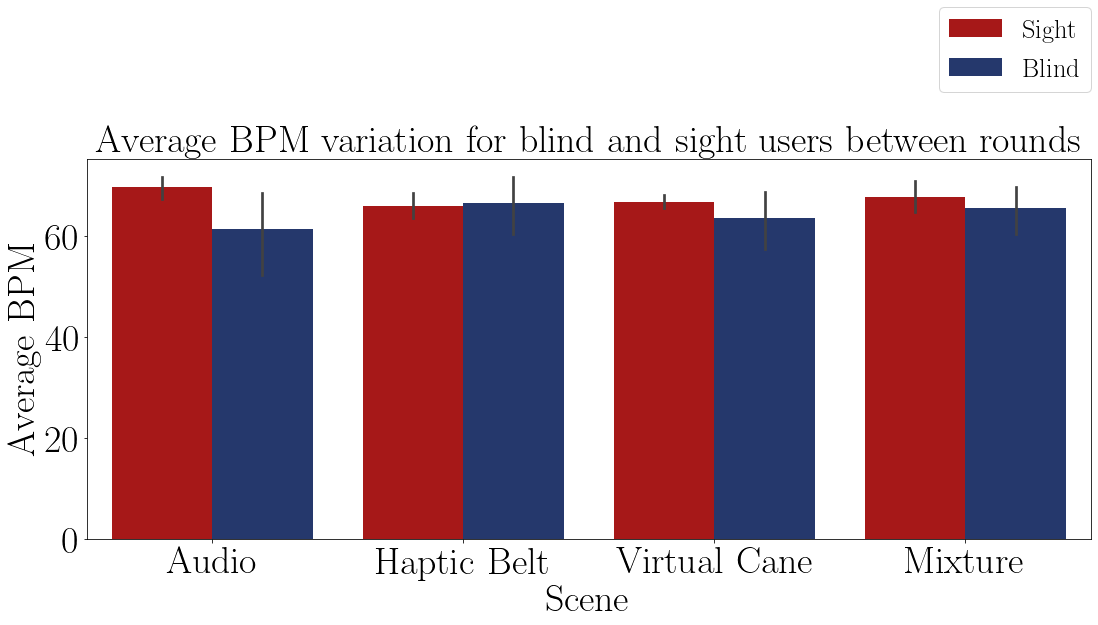
\includegraphics[width = 0.8\linewidth]{Resultados/ECG/Figuras/pdf/barplot_ecg_bpm_4_scene.pdf}
%    \caption{Barplot of the average BPM of both participants on each method.}
%    \label{fig:barplot_ecg_bpm_4_scene}
%\end{figure}

\begin{figure}[!htpb]
    \centering
    \begin{minipage}{0.45\textwidth}
        \centering
        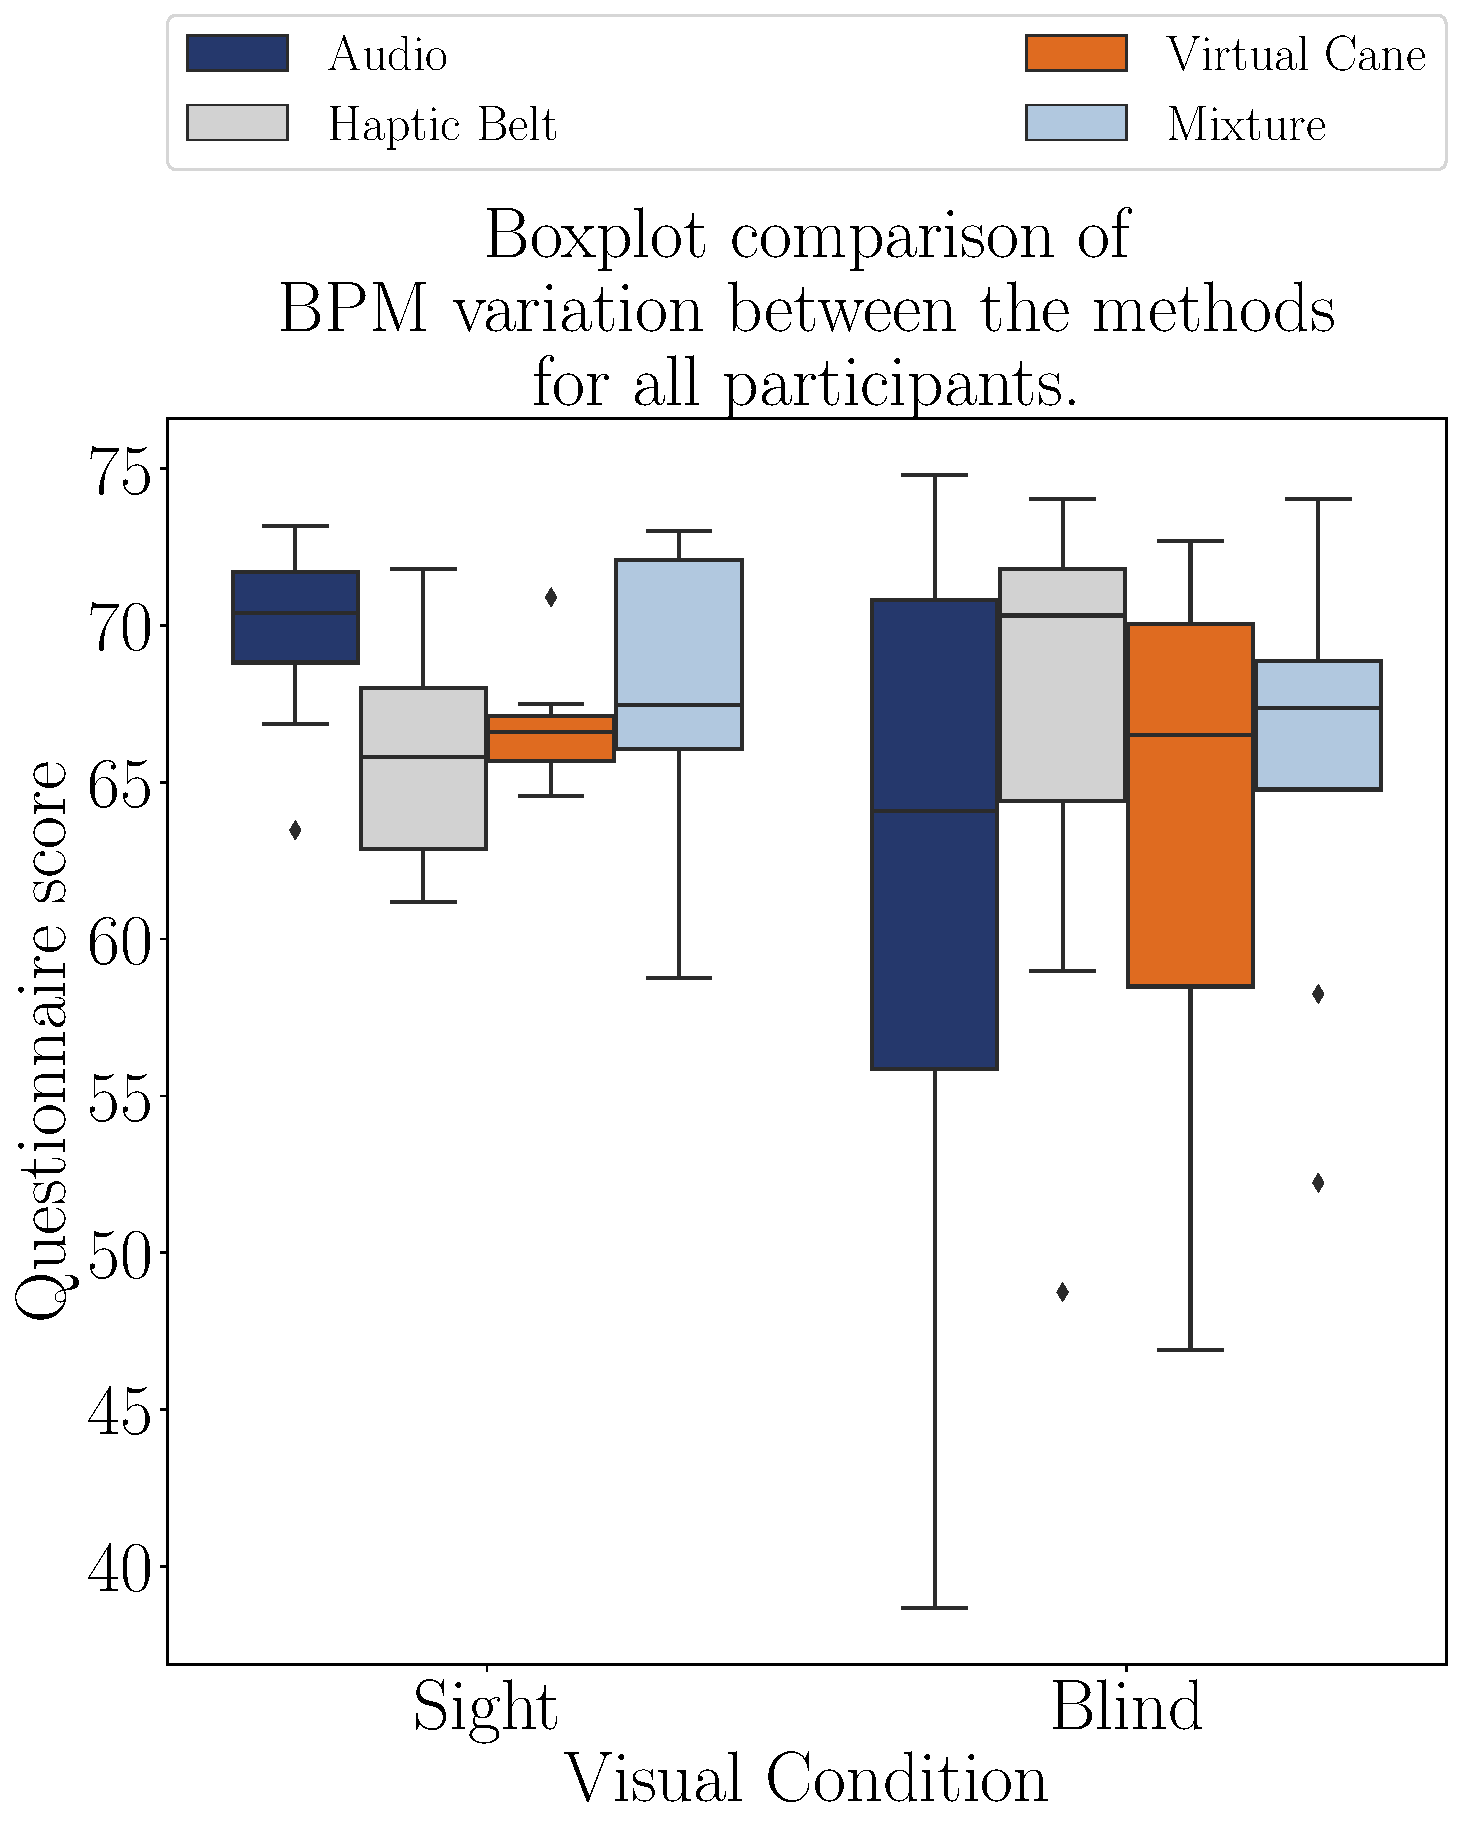
\includegraphics[width = 0.8\linewidth]{Resultados/ECG/Figuras/pdf/boxplot_ecg_bpm_4_scene.pdf}
        \caption{Boxplot of the average BPM of the participants grouped by method.}
        \label{fig:boxplot_ecg_bpm_4_scene}
    \end{minipage}
    \begin{minipage}{0.075\textwidth}
        \hfill
    \end{minipage}
    \begin{minipage}{0.45\textwidth}
        \centering
        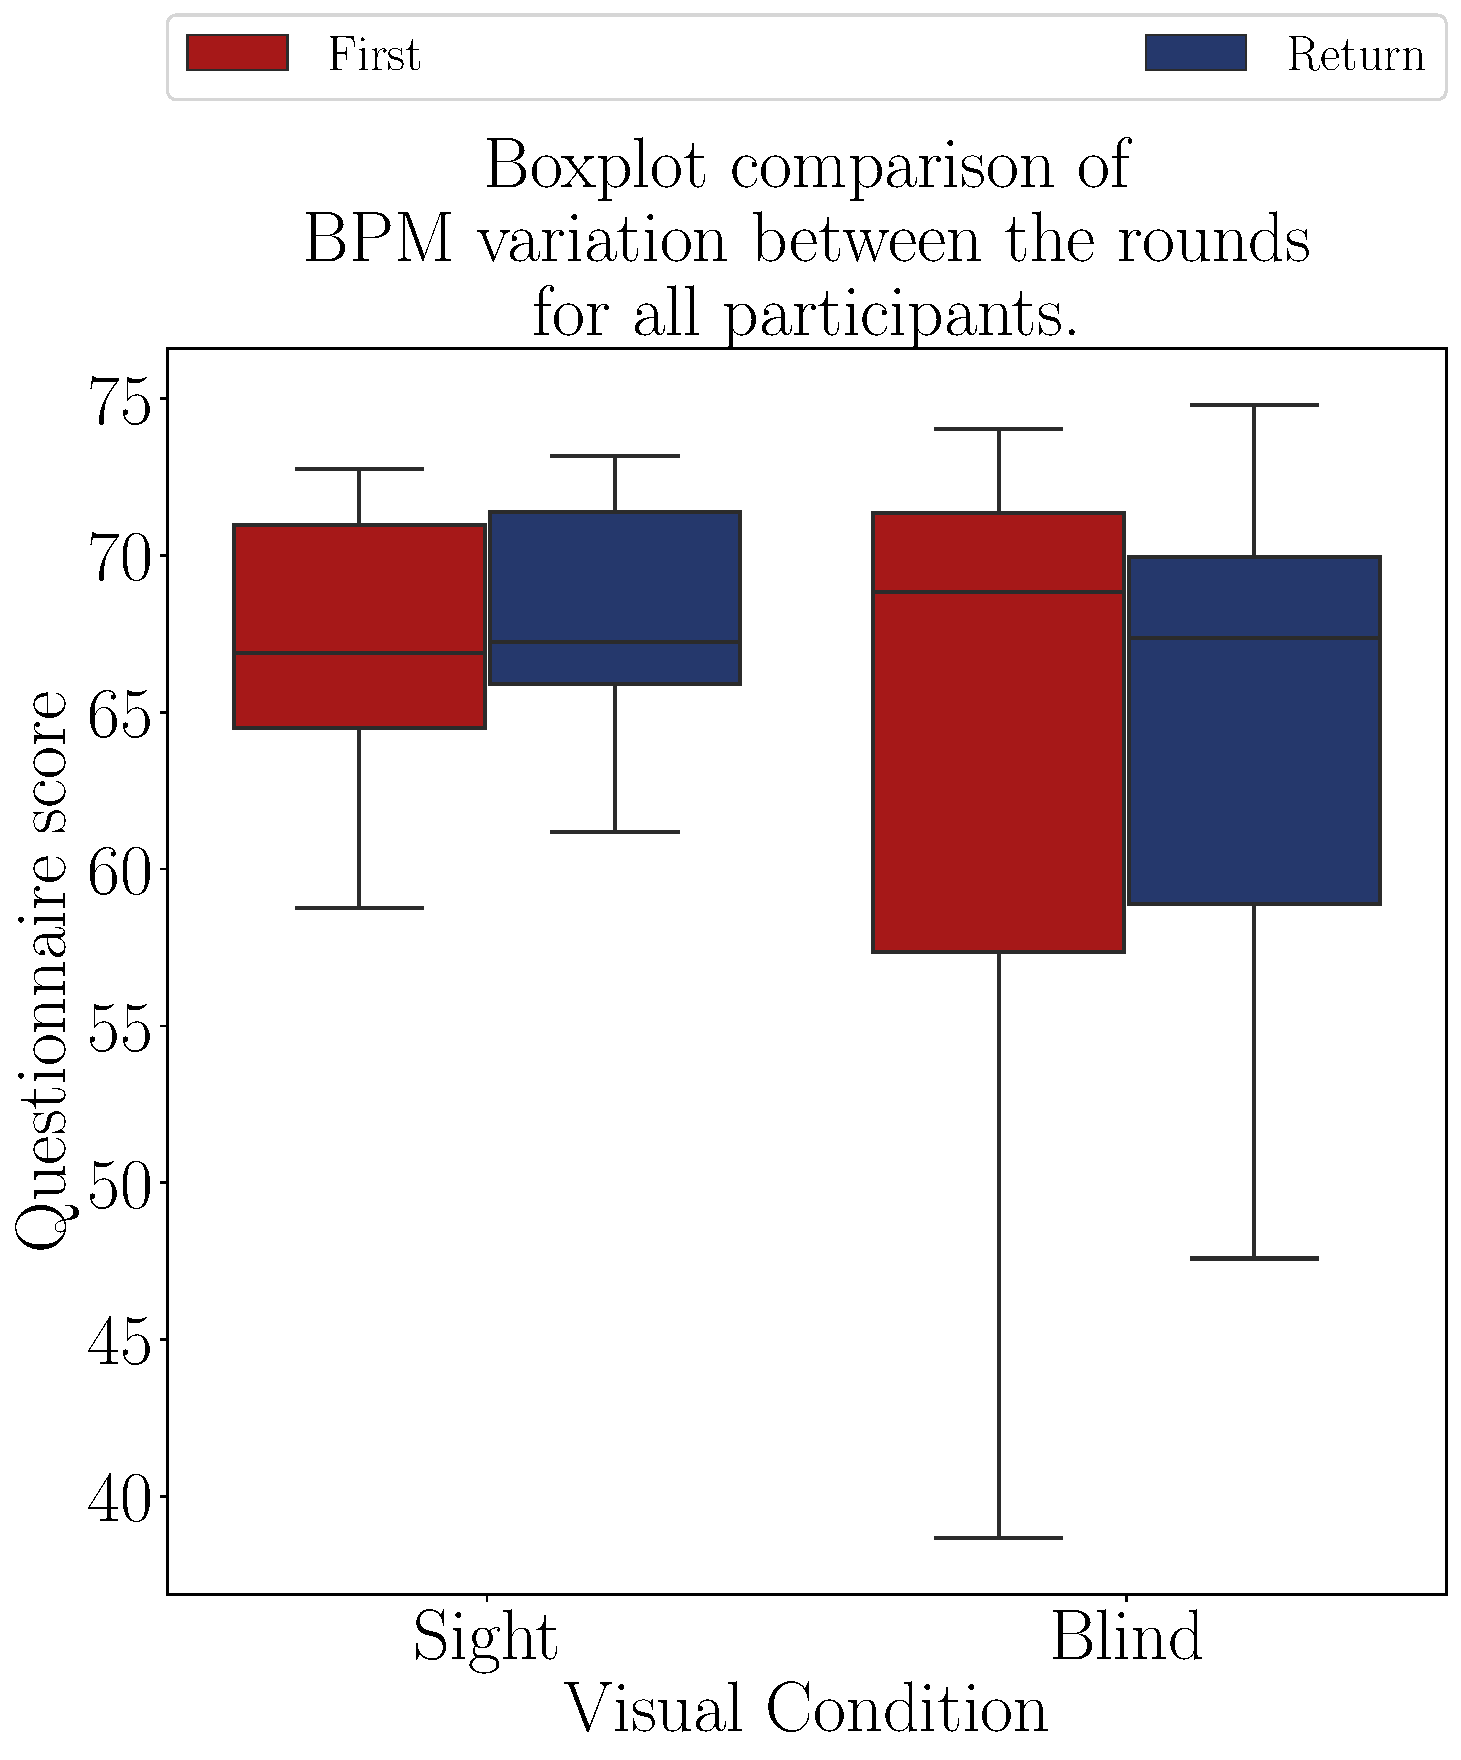
\includegraphics[width = 0.8\linewidth]{Resultados/ECG/Figuras/pdf/boxplot_ecg_bpm_4_rounds.pdf}
        \caption{Boxplot of the average BPM of the participants grouped by round.}
        \label{fig:boxplot_ecg_bpm_4_rounds}
    \end{minipage}
\end{figure}
 
%The Table \ref{tab:bpm_average_group_noBase} shows the average heartrate of both samples and is possible to notice how the average score by the blind users was higher in every method, apart of the "Haptic Belt".
%
%
\begin{table}[!htb]
\centering
\caption{ECG average BPM for each method grouped by visual condition.}
\label{tab:bpm_average_group_noBase}
\begin{tabular}{lllrrrr}
\toprule
{} &  Audio & Haptic Belt & Virtual Cane & Mixture \\
Visual Condition &        &             &              &         \\
\midrule
Blind            &  61.40 &       66.68 &        63.72 &   65.65 \\
Sight            &  69.73 &       66.03 &        66.75 &   67.88 \\
\bottomrule
\end{tabular}
\end{table}



The Figures \ref{fig:qqplot_bpm_two_way_sight} and \ref{fig:residplot_bpm_two_way_sight} shows the QQ plot and residual distributions for the sighted participants of the Table \ref{tab:bpm_table_noBase}. These figures shows that the data are normally distributed and that the methods have a similar variance. Table \ref{tab:blocanova_bpm_two_way_blind_sight} brings the results from ANOVA, which are similar for both sighted and blind participants.


\begin{table}[!htpb]
    \caption{Anova p-value for the BPM on each method.}
    \label{tab:blocanova_bpm_two_way_blind_sight}
\begin{minipage}{0.45\textwidth}
    \subcaption{Blind participants}
    \input{Resultados/ECG/Tabelas/blocanova_bpm_two_way_blindsemBegin.tex}
\end{minipage}
\begin{minipage}{0.45\textwidth}
    \subcaption{Sight participants}
    \input{Resultados/ECG/Tabelas/blocanova_bpm_two_way_sightsemBegin.tex}
\end{minipage}
\end{table}

\begin{figure}[!htpb]
    \centering
    %\vspace{-15.0cm}
    \begin{minipage}{0.45\textwidth}
        \centering
        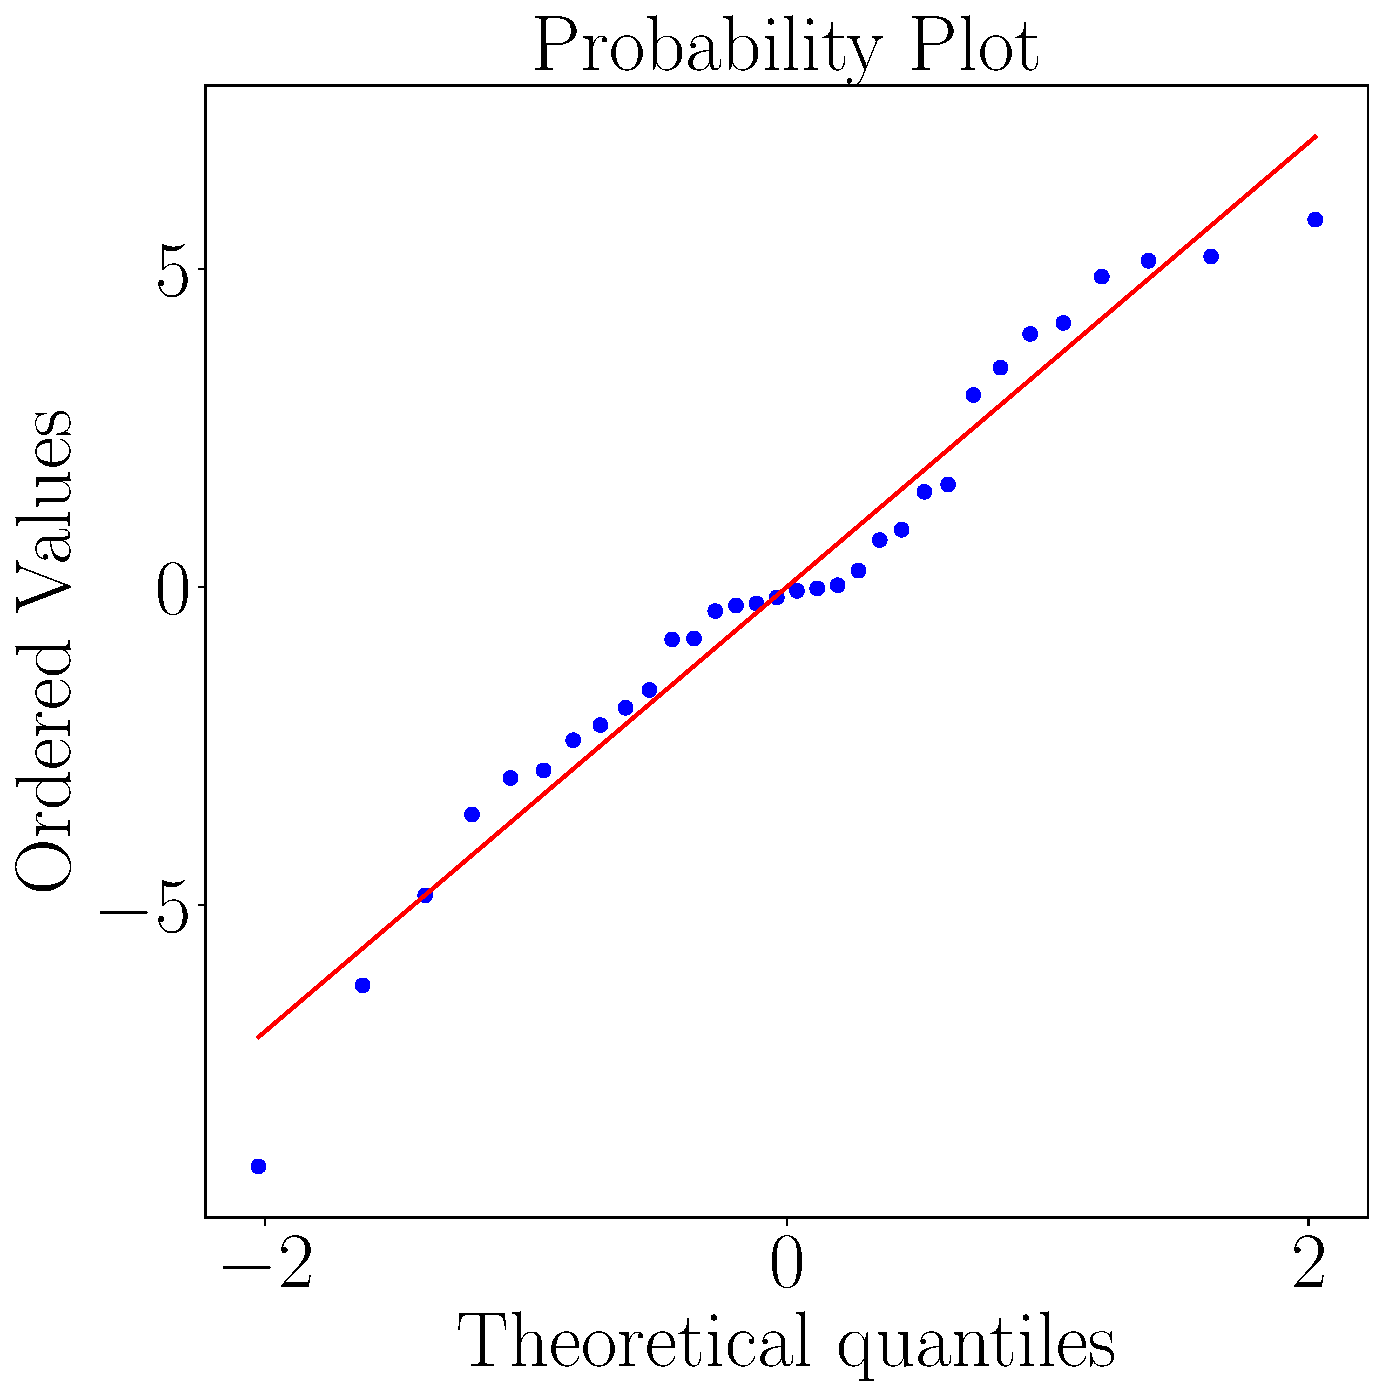
\includegraphics[width = 0.8\linewidth]{Resultados/ECG/Figuras/pdf/qqplot_bpm_two_way_sight.pdf}
        \caption{QQ plot of the BPM of the sight participants on each method.}
        \label{fig:qqplot_bpm_two_way_sight}
    \end{minipage}
    \begin{minipage}{0.075\textwidth}
        \hfill
    \end{minipage}
    \begin{minipage}{0.45\textwidth}
        \centering
        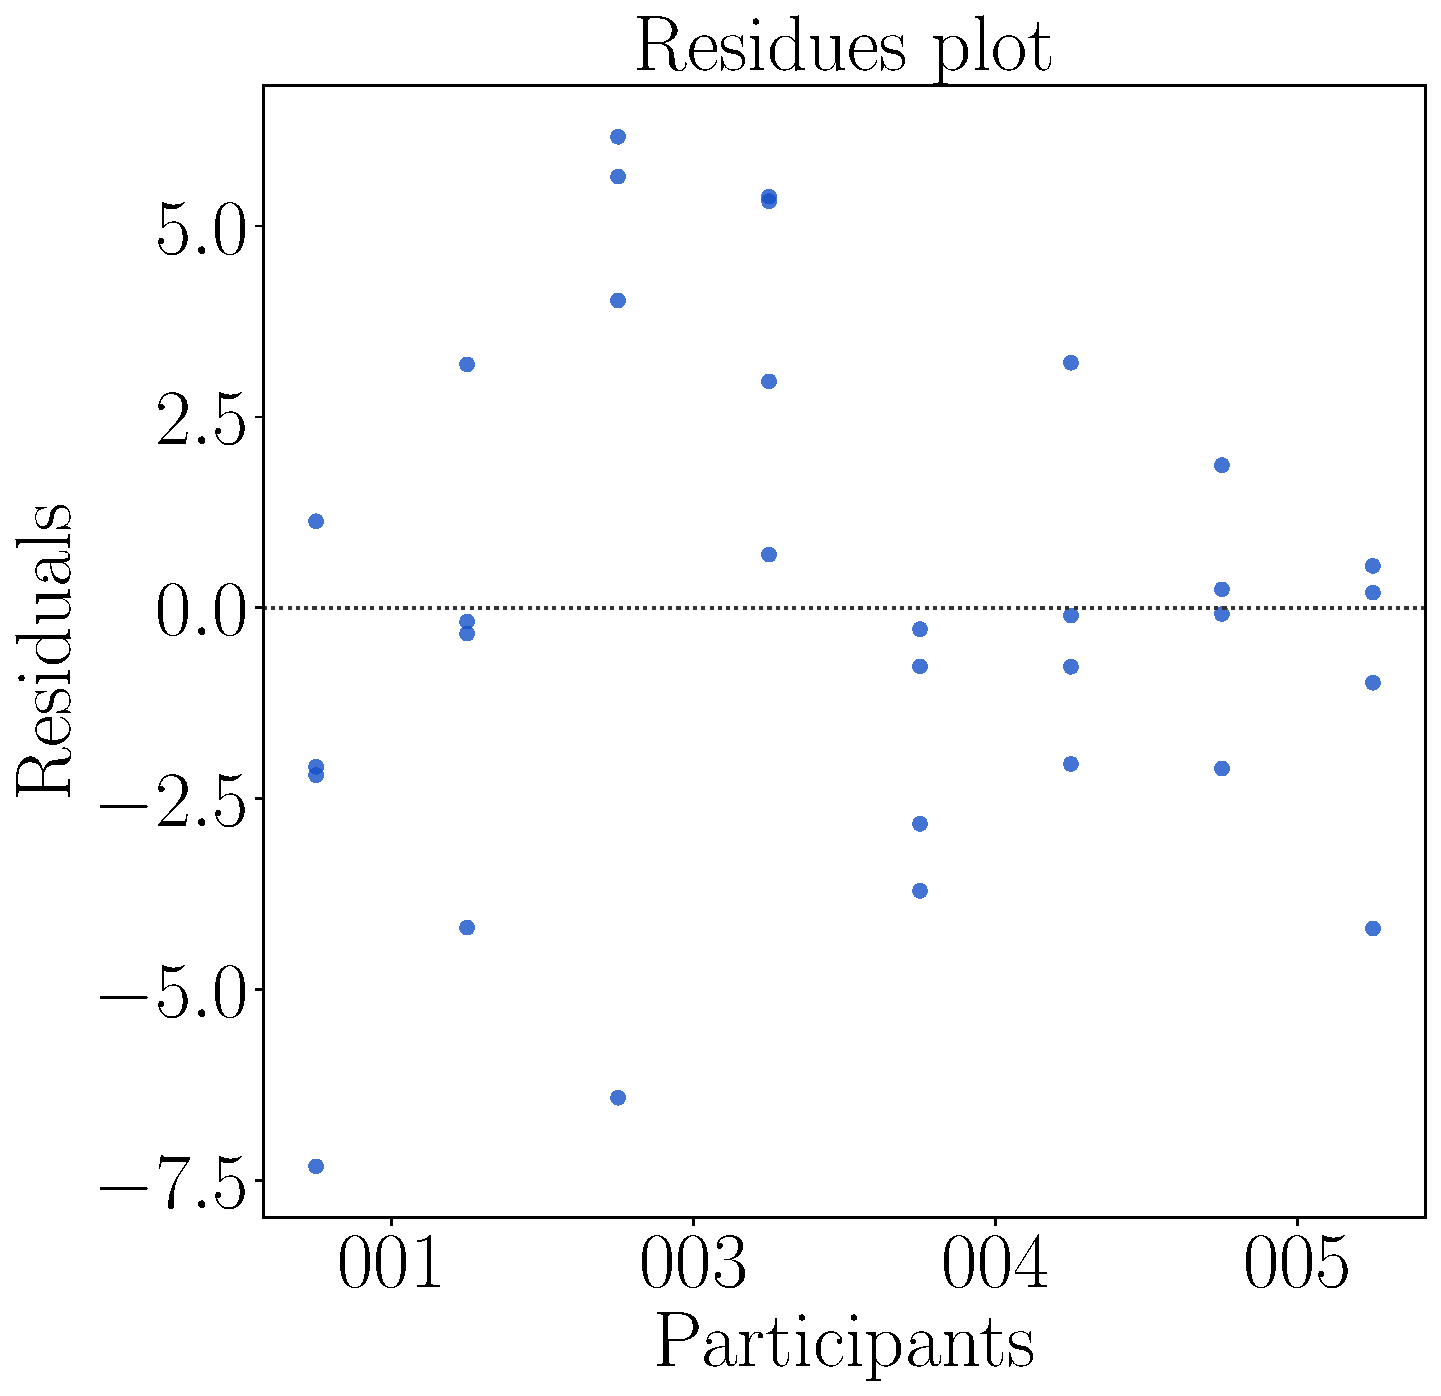
\includegraphics[width = 0.8\linewidth]{Resultados/ECG/Figuras/pdf/residplot_bpm_two_way_sight.pdf}
        \caption{Residual plot of the BPM score the sight participants on each method.}
        \label{fig:residplot_bpm_two_way_sight}
    \end{minipage}
\end{figure}

%
\begin{table}[!htb]
\centering
\caption{Cross validation p-value for the average BPM on each method for blinded users.}
\label{tab:lsd_bpm_two_way_sight}
\begin{tabular}{rclr}
\toprule
      \multicolumn{3}{c}{Method} &                          \multicolumn{2}{c}{Analysis} \\
\midrule
       Audio & $X$ & Haptic Belt &        $H_1 : \mu_{Audio} \ne \mu_{Haptic Belt}$ & ** \\
      Audio & $X$ & Virtual Cane &       $H_1 : \mu_{Audio} \ne \mu_{Virtual Cane}$ & ** \\
           Audio & $X$ & Mixture &            $H_1 : \mu_{Audio} \ne \mu_{Mixture}$ & ** \\
Haptic Belt & $X$ & Virtual Cane & $H_1 : \mu_{Haptic Belt} \ne \mu_{Virtual Cane}$ & ** \\
     Haptic Belt & $X$ & Mixture &      $H_1 : \mu_{Haptic Belt} \ne \mu_{Mixture}$ & ** \\
    Virtual Cane & $X$ & Mixture &     $H_1 : \mu_{Virtual Cane} \ne \mu_{Mixture}$ & ** \\
\bottomrule
\end{tabular}
\end{table}



%The Table \ref{tab:lsd_bpm_two_way_sight} presents the conclusion of a pairwise Fisher LSD test of the blind heart rate frequency variation between all the guidance methods and it shows that all methods had different effect on the heartrate.

%According to the ANOVA test at Table \ref{tab:blocanova_bpm_two_way_sight} there was no effect of the methods neither the rounds or their interaction, despite the fact that the Figure \ref{fig:boxplot_ecg_bpm_4_scene} showed a big difference between the methods. So the methods did not influence the sighted user mental workload. The same conclusion was driven in the section \ref{subsubsec:results_ecg_1} in the BPM part.

\FloatBarrier

%%%%%%%%%%%%%%%%%%%%%%%%%%%%%%%%%%%%%%%%%%%%%%%%%%%%%%%%%%%%%%%%%%%%%%%%%%%%
%%%%%%%%%%%%%%%%%%%%%%%%%%%%%%%%%%%%%%%%%%%%%%%%%%%%%%%%%%%%%%%%%%%%%%%%%%%%
%%%%%%%%%%%%%%%%%%%%%%%%%%%%%%%%%%%%%%%%%%%%%%%%%%%%%%%%%%%%%%%%%%%%%%%%%%%%
%%%%%%%%%%%%%%%%%%%%%%%%%%%%%%%%%%%%%%%%%%%%%%%%%%%%%%%%%%%%%%%%%%%%%%%%%%%%
%
%
\paragraph{Analysis of the heartbeat variance (SDNN)}\mbox{}\\
%

Table \ref{tab:sdnn_table_noBase} presents the SDNN for both sighted and blind participants. The mean values are presented in the barplots of Figure \ref{fig:barplot_ecg_sdnn_4_scene_blind_sight}.


\begin{table}[!htb]
\centering
\caption{Average SDNN by the participants during the each round and method [ms].}
\label{tab:sdnn_table_noBase}
\begin{tabular}{lllrrrrr}
\toprule
    &       &        &   Audio &  \begin{tabular}[c]{@{}l@{}}Haptic\\ Belt\end{tabular} &  \begin{tabular}[c]{@{}l@{}}Virtual\\ Cane\end{tabular} &  Mixture \\
Part. & \begin{tabular}[c]{@{}l@{}}Visual\\ Condition\end{tabular} & Round &         &                                                        &                                                         &          \\
\midrule
001C & Blind & First & 107.061 &                                                124.737 &                                                 163.968 &  129.054 \\
    &       & Return & 130.885 &                                                131.590 &                                                 157.589 &  124.786 \\
002C & Blind & First &  98.863 &                                                 81.140 &                                                  33.977 &   79.289 \\
    &       & Return &  49.627 &                                                 42.815 &                                                 114.057 &  107.545 \\
003C & Blind & First &  38.325 &                                                 35.101 &                                                  42.392 &   43.692 \\
    &       & Return &  41.196 &                                                 44.256 &                                                  42.602 &   46.145 \\
004C & Blind & First &  86.827 &                                                 62.560 &                                                  85.900 &   70.472 \\
    &       & Return &  74.895 &                                                 70.017 &                                                  66.089 &  104.040 \\
001 & Sight & First &  82.185 &                                                134.530 &                                                 134.773 &  225.408 \\
    &       & Return &  69.479 &                                                318.747 &                                                 116.003 &  136.507 \\
003 & Sight & First &  79.600 &                                                 51.782 &                                                  68.676 &   60.842 \\
    &       & Return &  45.709 &                                                 40.927 &                                                  66.323 &   47.823 \\
004 & Sight & First & 121.130 &                                                154.718 &                                                 128.477 &  125.947 \\
    &       & Return & 100.366 &                                                122.563 &                                                 140.115 &  119.260 \\
005 & Sight & First &  87.686 &                                                120.522 &                                                  88.591 &  102.796 \\
    &       & Return &  93.207 &                                                122.839 &                                                 141.305 &   96.035 \\
\bottomrule
\end{tabular}
\end{table}



\begin{figure}[!htpb]
    \centering
    \begin{minipage}{\textwidth}
        \centering
        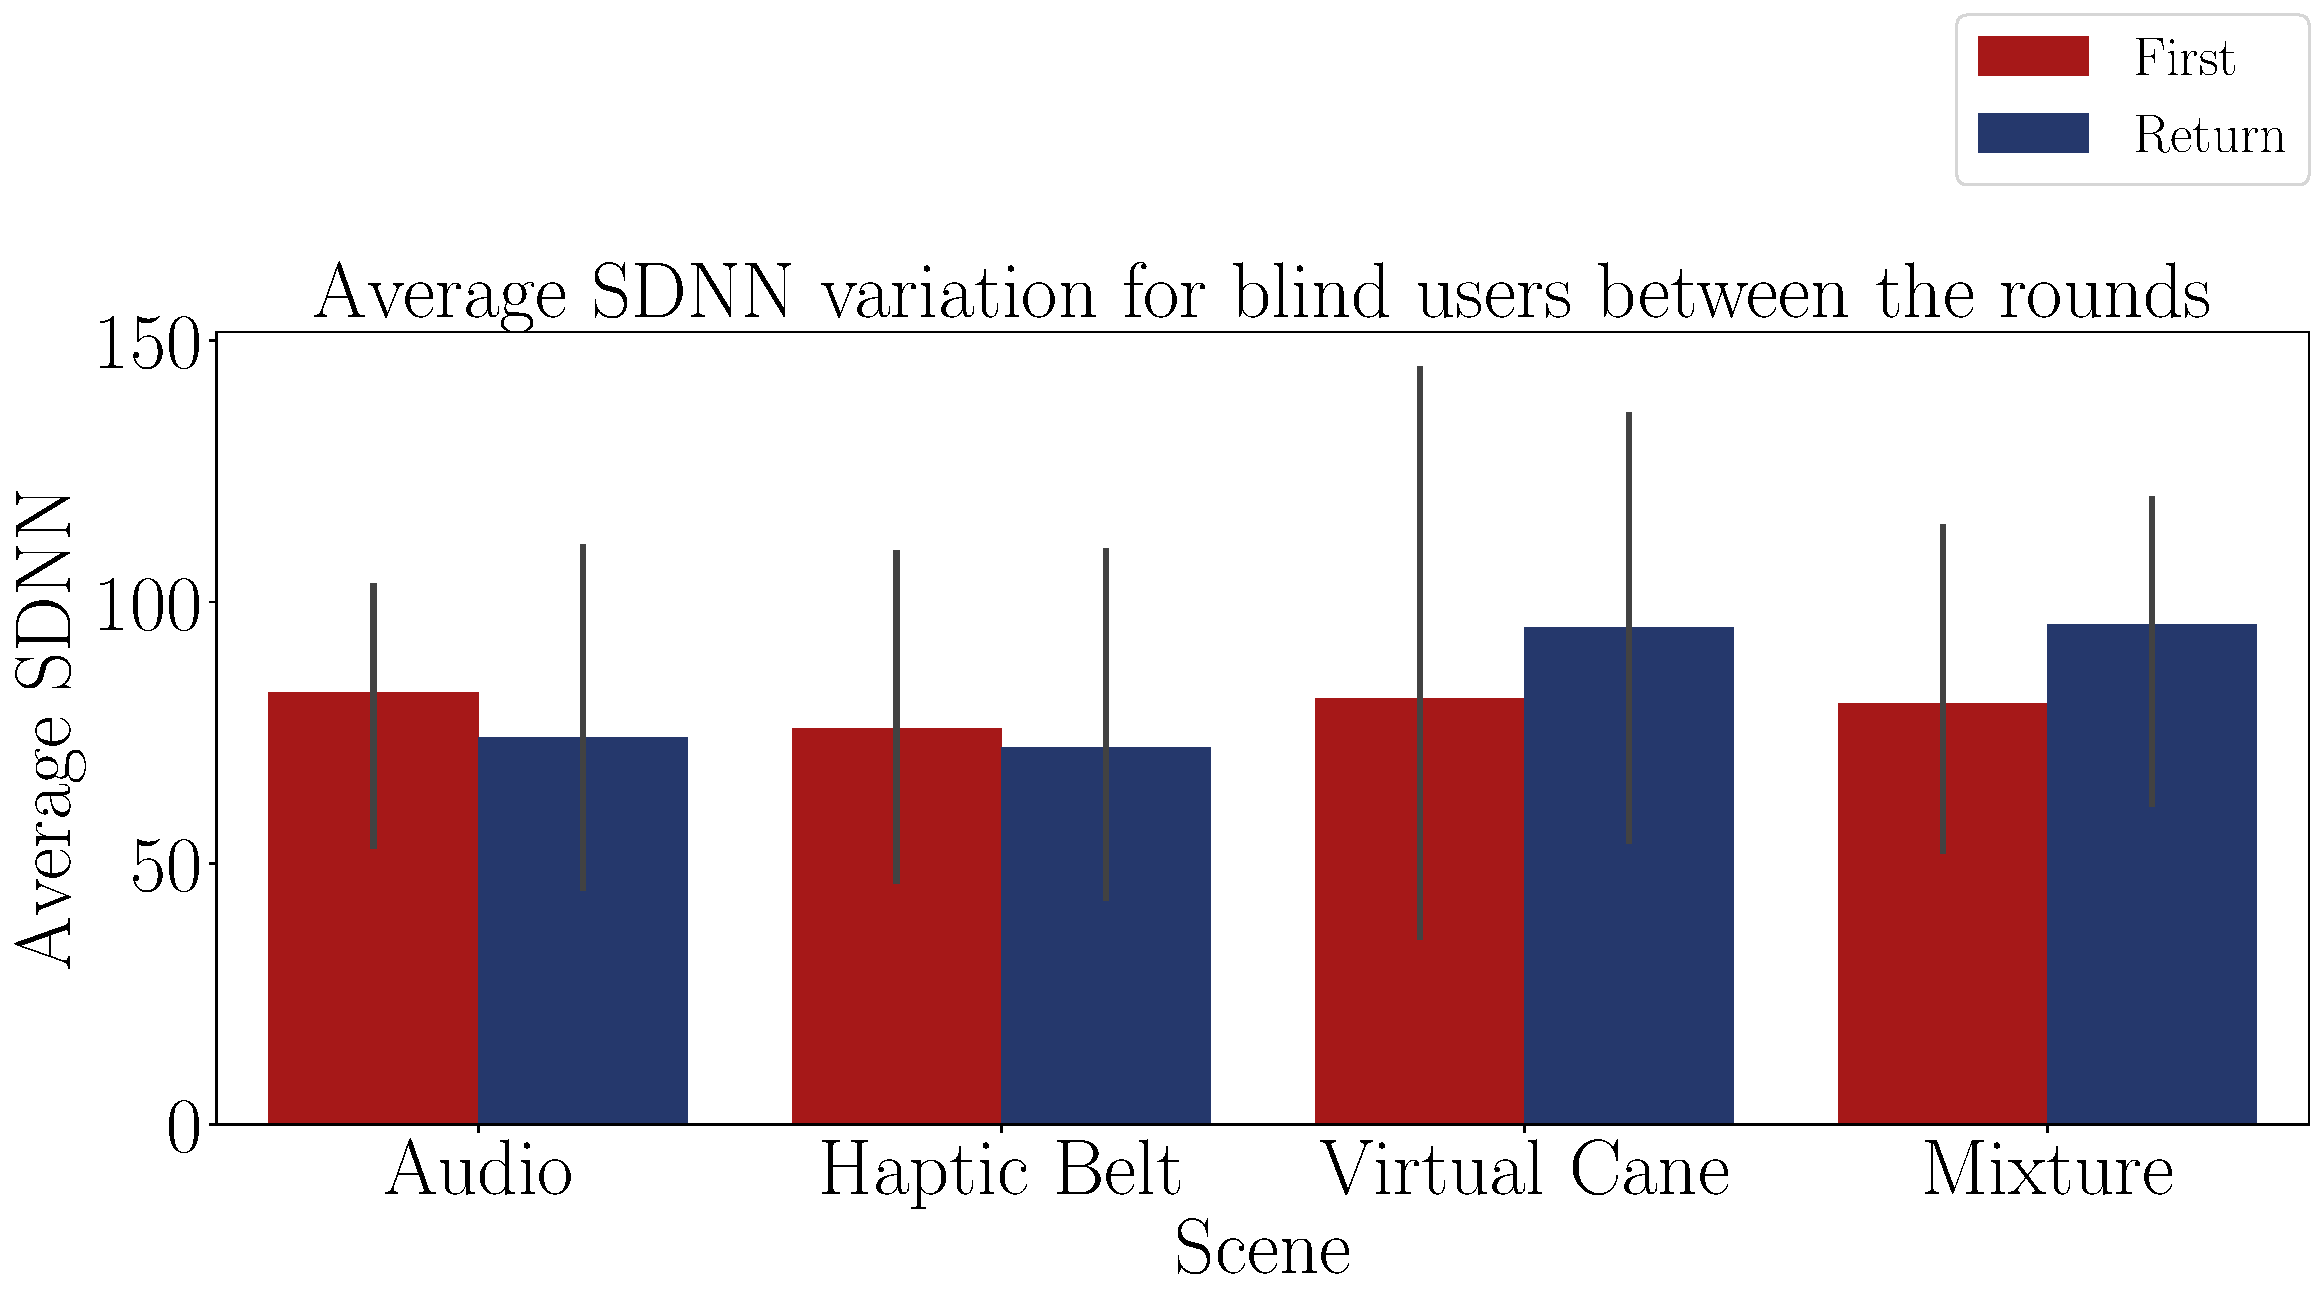
\includegraphics[width = 0.8\linewidth]{Resultados/ECG/Figuras/pdf/barplot_ecg_sdnn_4_scene_blind.pdf}
        \subcaption{Blind participants.}
        \label{fig:barplot_ecg_sdnn_4_scene_blind}
    \end{minipage}
    \begin{minipage}{\textwidth}
        \centering
        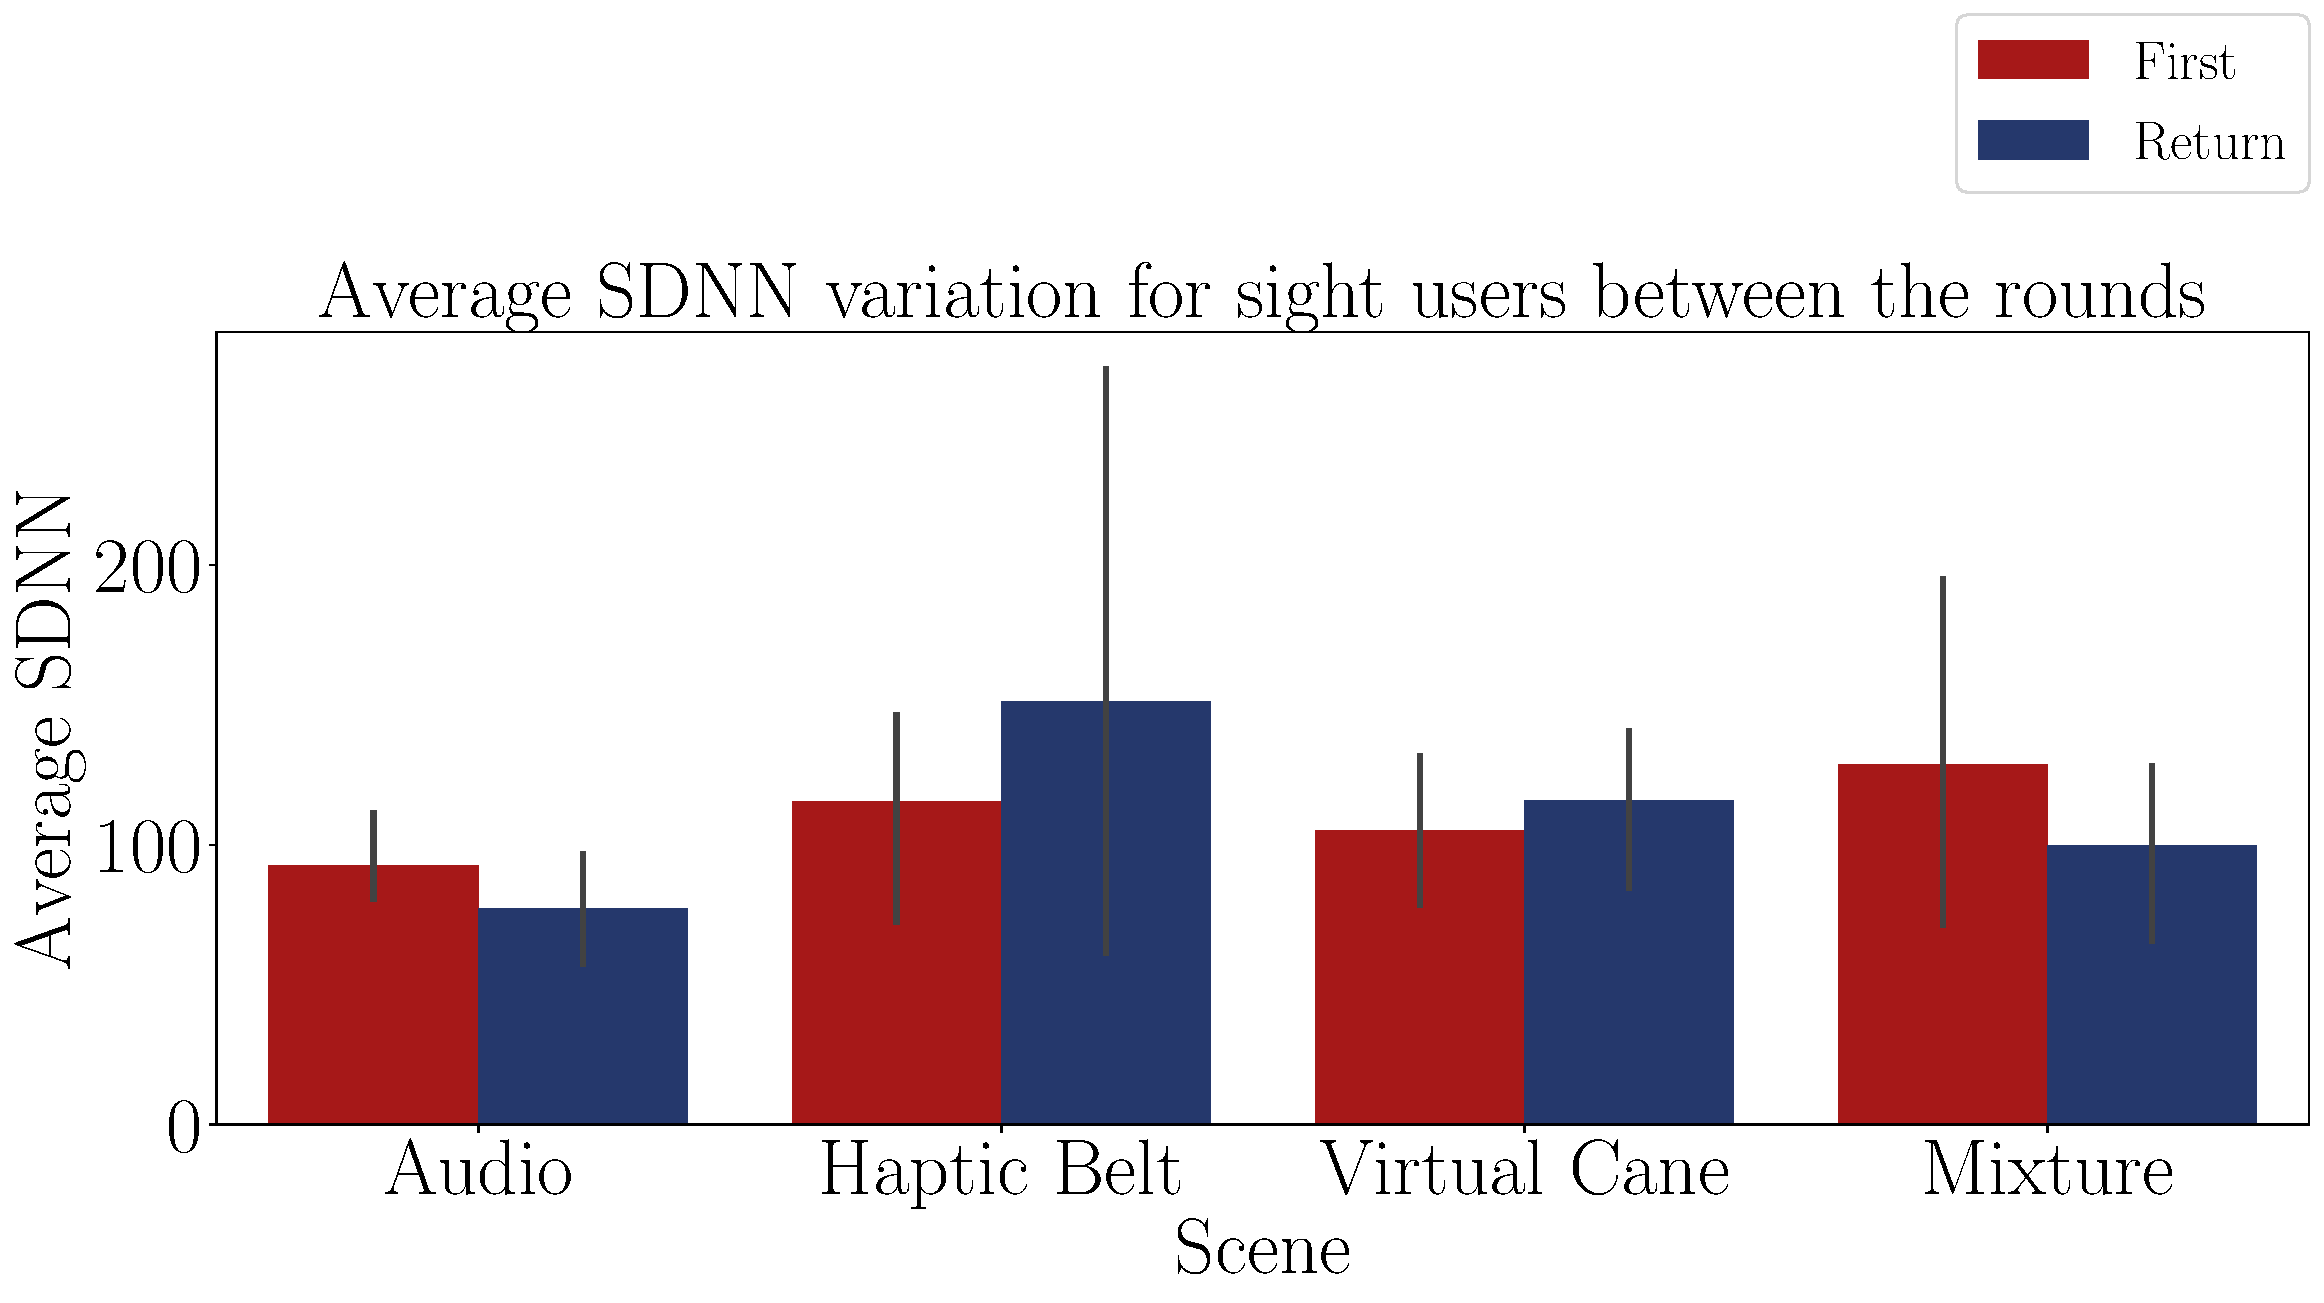
\includegraphics[width = 0.8\linewidth]{Resultados/ECG/Figuras/pdf/barplot_ecg_sdnn_4_scene_sight.pdf}
        \subcaption{Sight participants.}
        \label{fig:barplot_ecg_sdnn_4_scene_sight}
    \end{minipage}
    \caption{Barplot of the average SDNN of the on each method and round.}
    \label{fig:barplot_ecg_sdnn_4_scene_blind_sight}
\end{figure}
%\begin{figure}[!htpb]
%    \centering
%    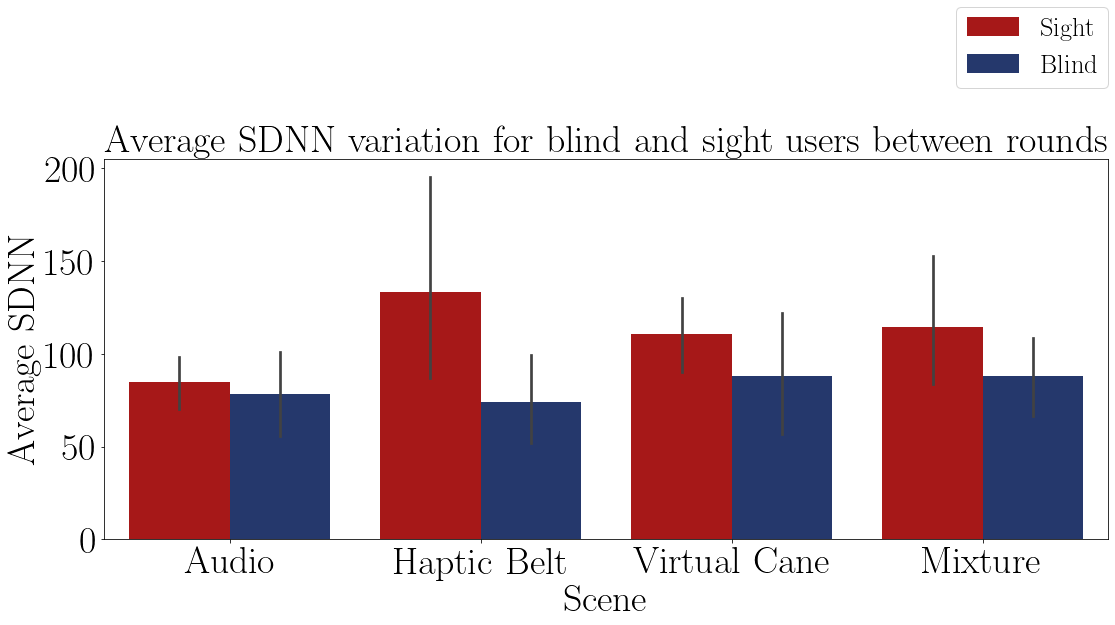
\includegraphics[width = 0.8\linewidth]{Resultados/ECG/Figuras/pdf/barplot_ecg_sdnn_4_scene.pdf}
%    \caption{Barplot of the average SDNN of both participants on each method.}
%    \label{fig:barplot_ecg_sdnn_4_scene}
%\end{figure}

No clear pattern is evident from this figure. For some methods, the return round resulted in a decrease of the SDNN while for others, it increased. 

Figures \ref{fig:boxplot_ecg_sdnn_4_scene} and \ref{fig:boxplot_ecg_sdnn_4_rounds} shows the boxplots for both groups. Both pictures show that the SDNN of the sighted users were higher than that of the blind users, indicating that sighted users had a lower mental workload than the blind users.

\begin{figure}[!htpb]
    \centering
    \begin{minipage}{0.45\textwidth}
        \centering
        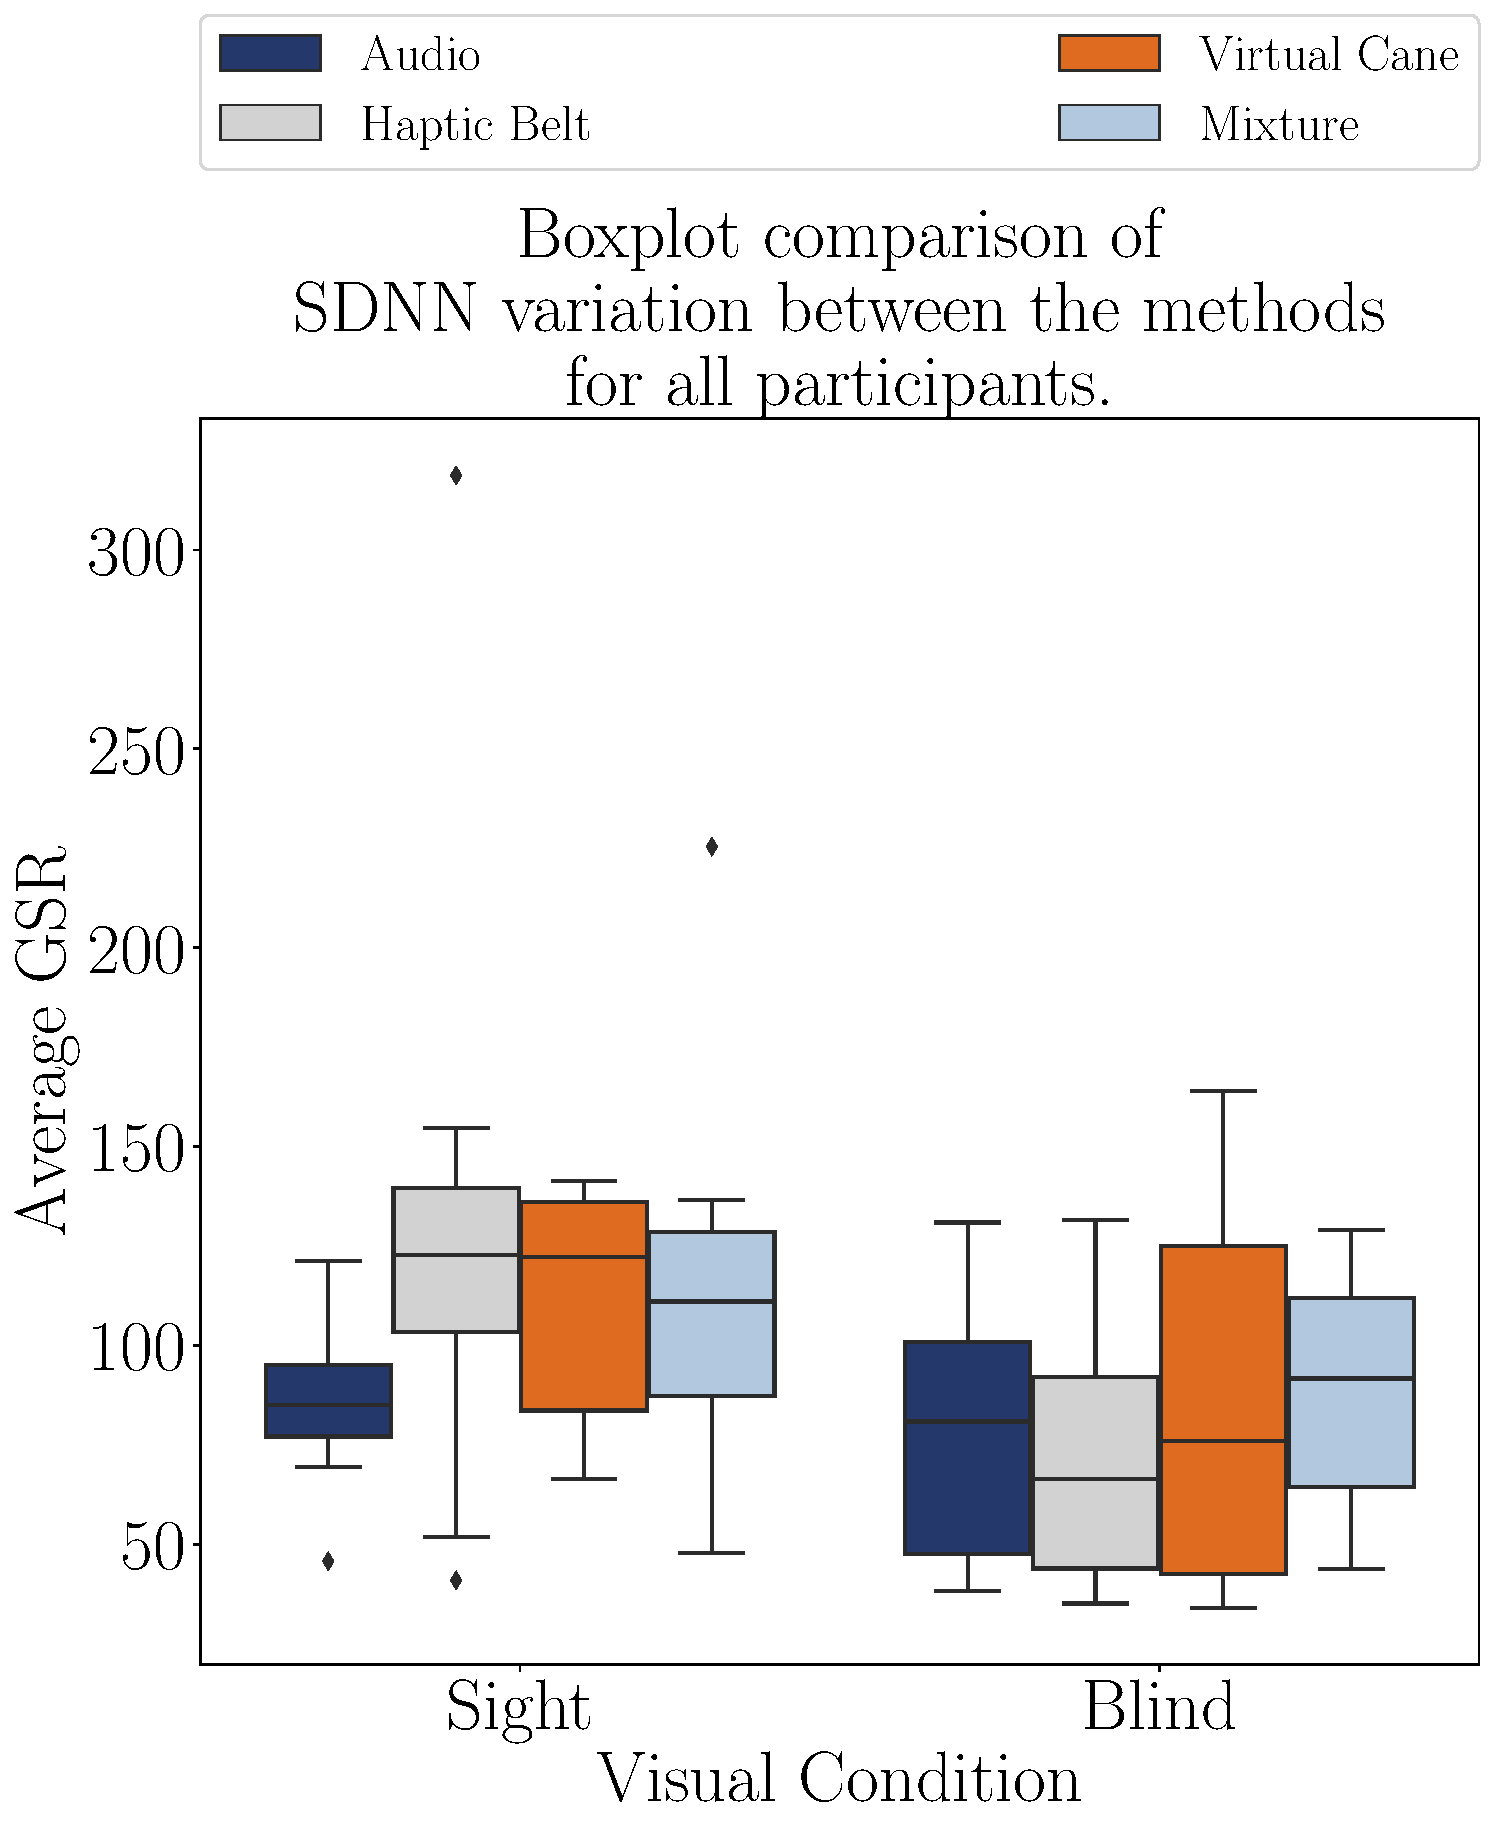
\includegraphics[width = 0.8\linewidth]{Resultados/ECG/Figuras/pdf/boxplot_ecg_sdnn_4_scene.pdf}
        \caption{Boxplot of the average SDNN of the participants grouped by method.}
        \label{fig:boxplot_ecg_sdnn_4_scene}
    \end{minipage}
    \begin{minipage}{0.075\textwidth}
        \hfill
    \end{minipage}
    \begin{minipage}{0.45\textwidth}
        \centering
        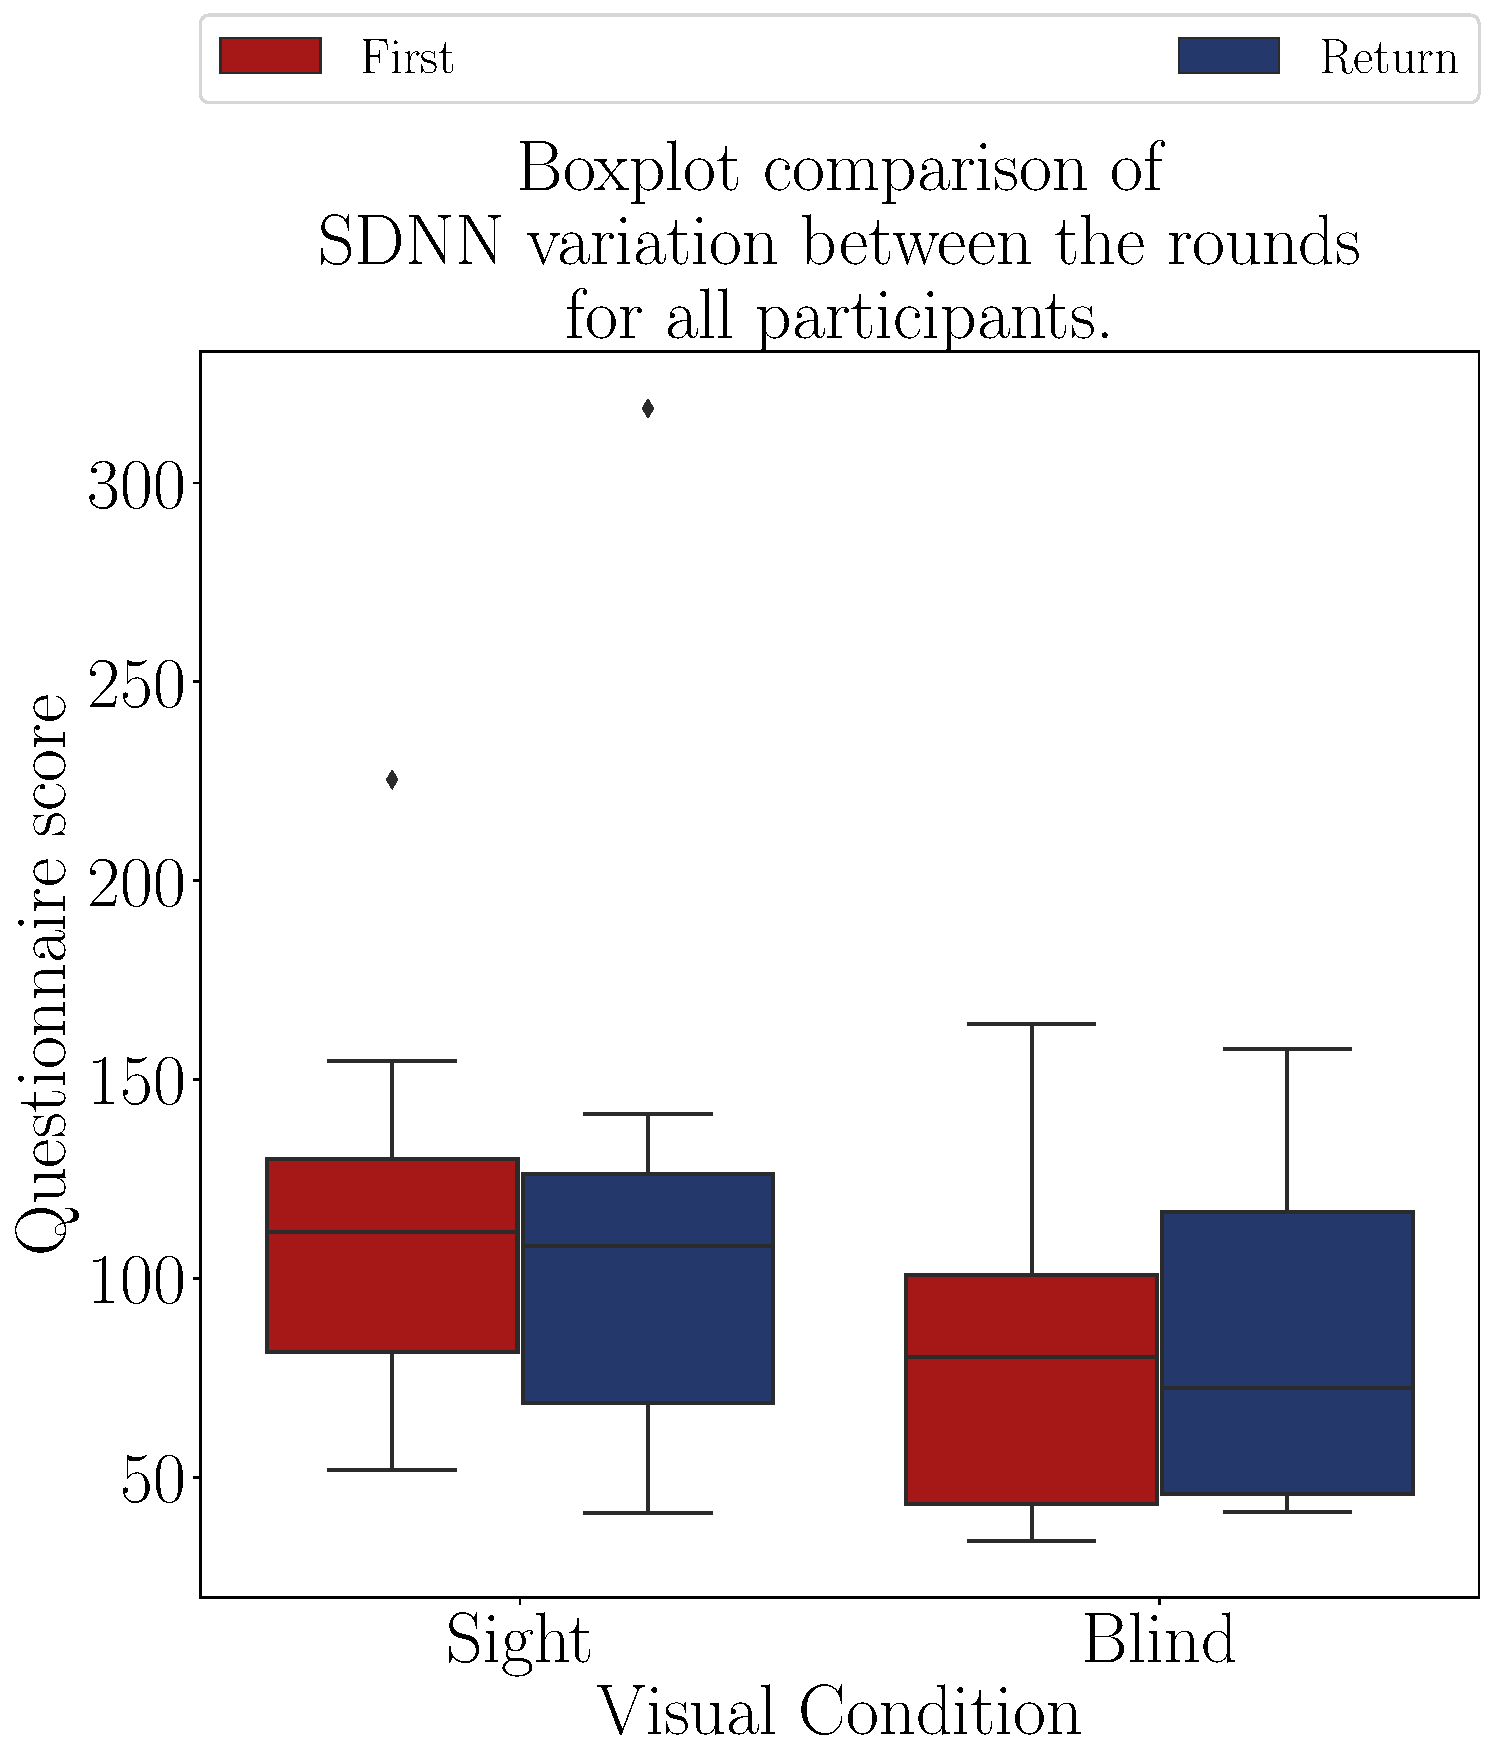
\includegraphics[width = 0.8\linewidth]{Resultados/ECG/Figuras/pdf/boxplot_ecg_sdnn_4_rounds.pdf}
        \caption{Boxplot of the average SDNN of the participants grouped by round.}
        \label{fig:boxplot_ecg_sdnn_4_rounds}
    \end{minipage}
\end{figure}
 
%The Table \ref{tab:sdnn_average_group_noBase} shows the average heartbeat variance of both samples and is possible to notice how the average score by the sight users was higher in every method, reinforcing the Figures \ref{fig:barplot_ecg_sdnn_4_scene} to \ref{fig:boxplot_ecg_sdnn_4_rounds} conclusions.
%
%
\begin{table}[!htb]
\centering
\caption{ECG Average SDNN average in relation to the baseline grouped by participant and visual Condition.}
\label{tab:sdnn_average_group_noBase}
\begin{tabular}{lllrrrr}
\toprule
{} &  Audio & Haptic Belt & Virtual Cane & Mixture \\
Visual Condition &        &             &              &         \\
\midrule
Blind            &  78.46 &       74.03 &        88.32 &   88.13 \\
Sight            &  84.92 &      133.33 &       110.53 &  114.33 \\
\bottomrule
\end{tabular}
\end{table}



Figures \ref{fig:qqplot_sdnn_two_way_sight} and \ref{fig:residplot_sdnn_two_way_sight} bring the QQ Plot and residual distribution. Figure \ref{fig:qqplot_sdnn_two_way_sight} hints that the data from sighted users contain two outliers. Table \ref{tab:blocanova_sdnn_two_way_blind_sight} shows the ANOVA test p-values. For both groups, none of the factors have a significant influence on the SDNN value.

\begin{table}[!htpb]
    \caption{Anova p-value for the average SDNN on each method.'}
    \label{tab:blocanova_sdnn_two_way_blind_sight}
\begin{minipage}{0.45\textwidth}
    \subcaption{Blind participants}
    \input{Resultados/ECG/Tabelas/blocanova_sdnn_two_way_blindsemBegin.tex}
\end{minipage}
\begin{minipage}{0.45\textwidth}
    \subcaption{Sight participants}
    \input{Resultados/ECG/Tabelas/blocanova_sdnn_two_way_sightsemBegin.tex}
\end{minipage}
\end{table}

\begin{figure}[!htpb]
    \centering
    %\vspace{-15.0cm}
    \begin{minipage}{0.45\textwidth}
        \centering
        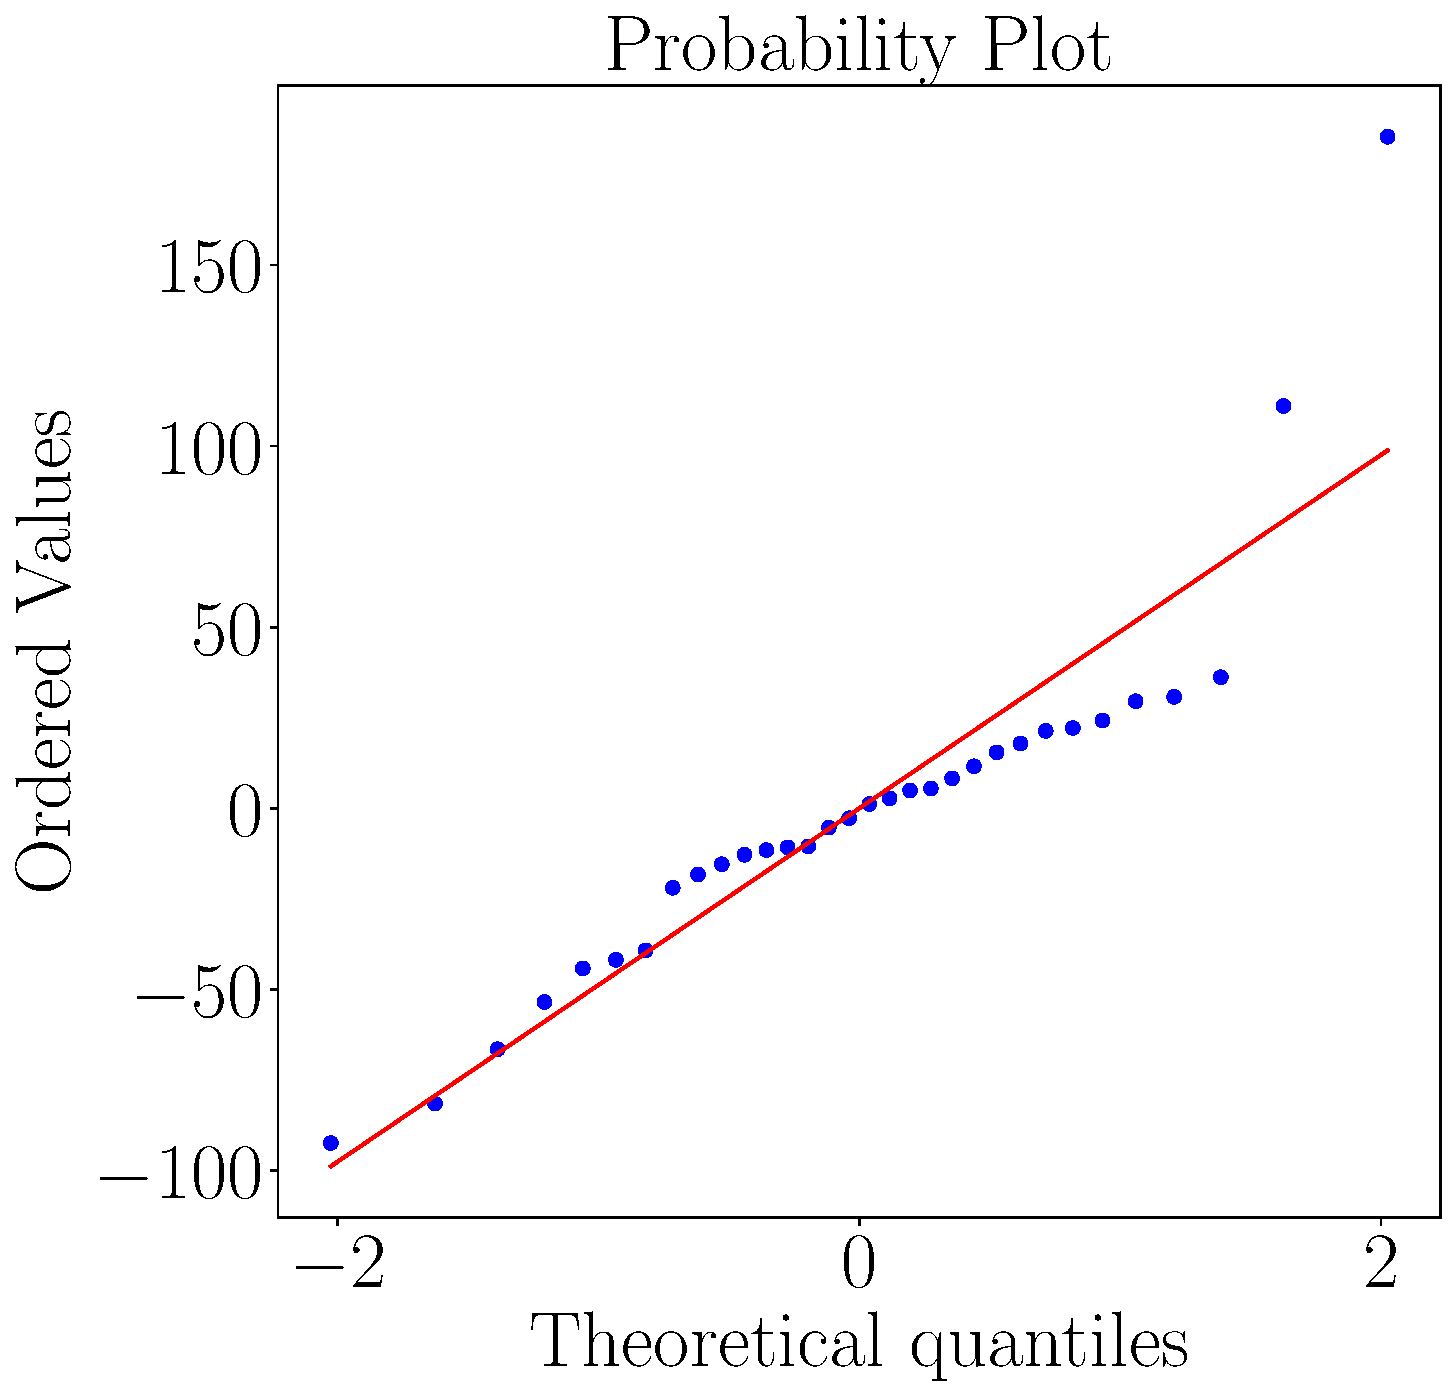
\includegraphics[width = 0.8\linewidth]{Resultados/ECG/Figuras/pdf/qqplot_sdnn_two_way_sight.pdf}
        \caption{QQ plot of the average SDNN of the sight participants on each method.}
        \label{fig:qqplot_sdnn_two_way_sight}
    \end{minipage}
    \begin{minipage}{0.075\textwidth}
        \hfill
    \end{minipage}
    \begin{minipage}{0.45\textwidth}
        \centering
        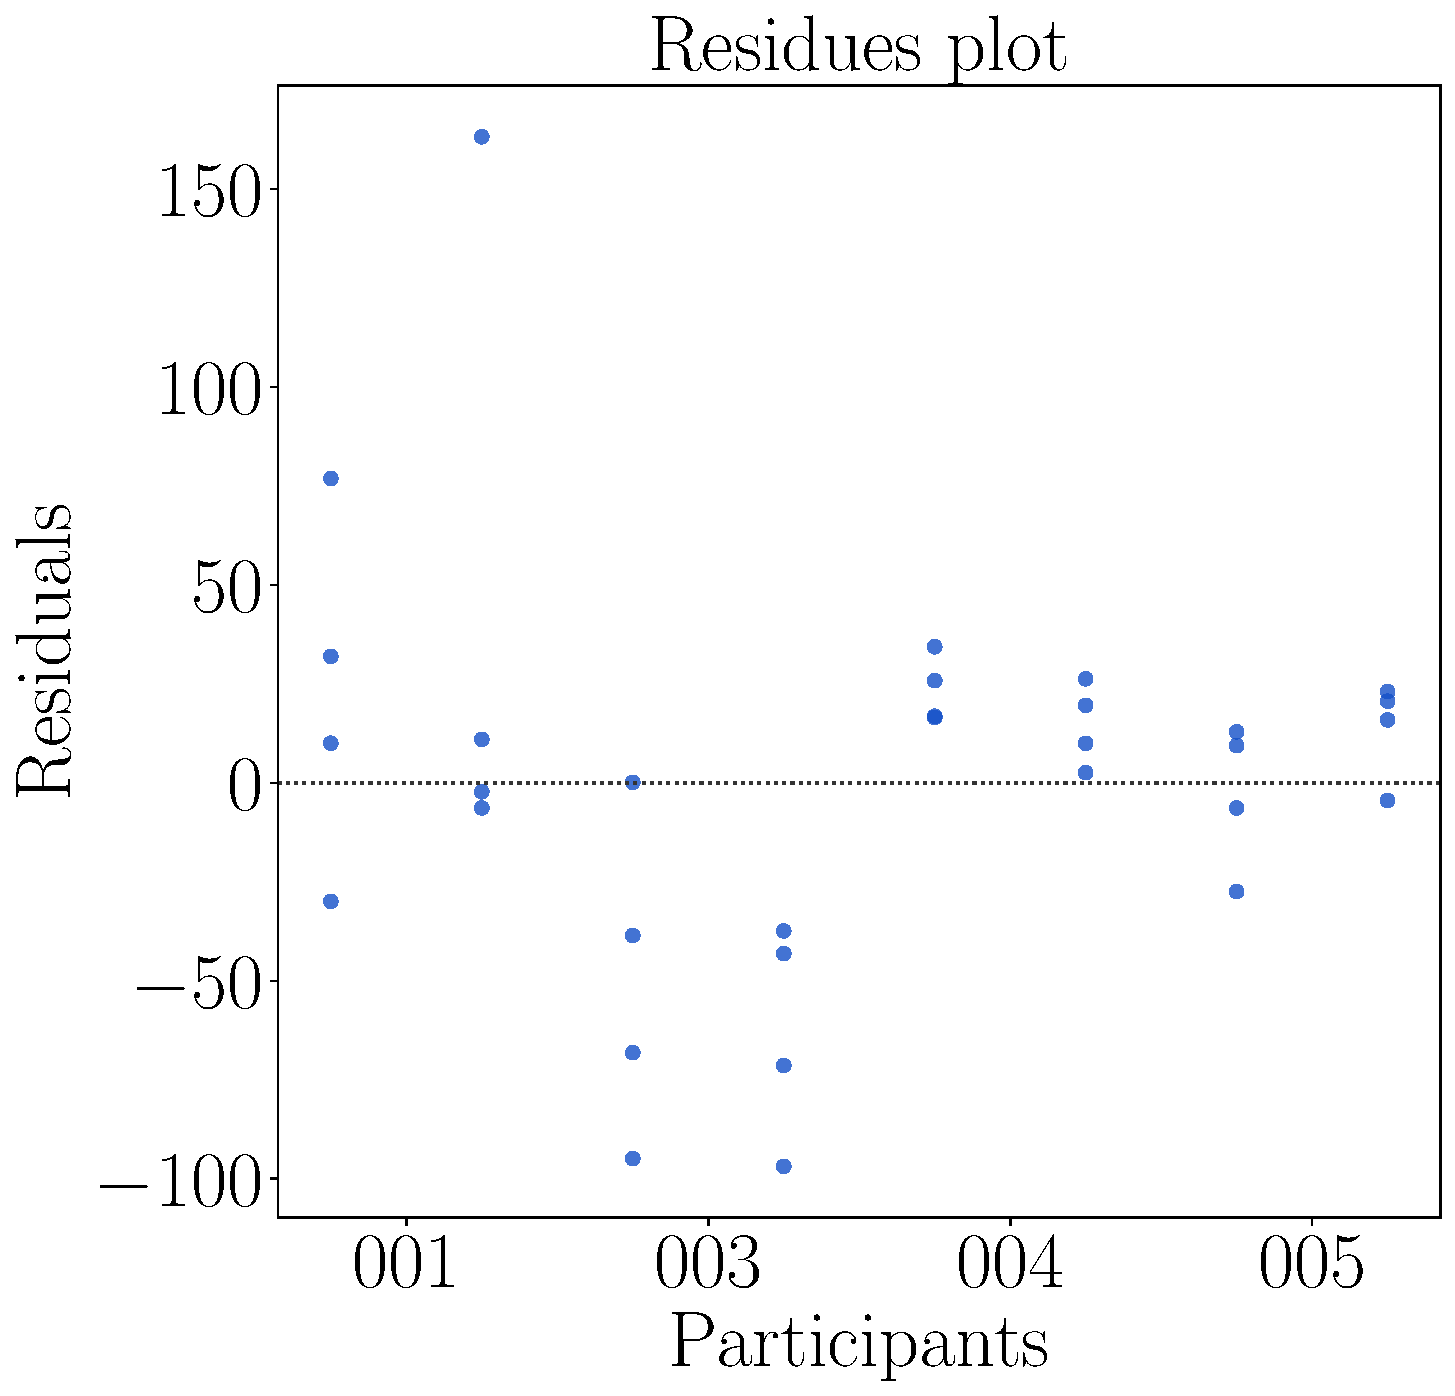
\includegraphics[width = 0.8\linewidth]{Resultados/ECG/Figuras/pdf/residplot_sdnn_two_way_sight.pdf}
        \caption{Residual plot of the average SDNN score the sight participants on each method.}
        \label{fig:residplot_sdnn_two_way_sight}
    \end{minipage}
\end{figure}


%
\begin{table}[!htb]
\centering
\caption{Cross validation p-value for the average SDNN on each method for blinded users.}
\label{tab:lsd_sdnn_two_way_sight}
\begin{tabular}{rclr}
\toprule
      \multicolumn{3}{c}{Method} &                          \multicolumn{2}{c}{Analysis} \\
\midrule
       Audio & $X$ & Haptic Belt &        $H_1 : \mu_{Audio} \ne \mu_{Haptic Belt}$ & ** \\
      Audio & $X$ & Virtual Cane &       $H_1 : \mu_{Audio} \ne \mu_{Virtual Cane}$ & ** \\
           Audio & $X$ & Mixture &            $H_1 : \mu_{Audio} \ne \mu_{Mixture}$ & ** \\
Haptic Belt & $X$ & Virtual Cane & $H_1 : \mu_{Haptic Belt} \ne \mu_{Virtual Cane}$ & ** \\
     Haptic Belt & $X$ & Mixture &      $H_1 : \mu_{Haptic Belt} \ne \mu_{Mixture}$ & ** \\
    Virtual Cane & $X$ & Mixture &         $H_0 : \mu_{Virtual Cane} = \mu_{Mixture}$ &  \\
\bottomrule
\end{tabular}
\end{table}


%
%The Table \ref{tab:lsd_sdnn_two_way_sight} presents the conclusion of a pairwise Fisher LSD test of the blind heart rate frequency variation between all the guidance methods and it shows that all methods had different effect on the heartrate, appart of the "Virtual Cane" and "Mixture", which presented similar SDNN.

%According to the ANOVA test at Table \ref{tab:blocanova_sdnn_two_way_sight} there was no effect on the interbeat variance. So the methods did not influence the sighted user mental workload. The same conclusion was driven in the section \ref{subsubsec:results_ecg_1} in the SDNN part.
%
%Also, the sight user had a higher SDNN, which means lower Mental Workload, a unexpected result based on the expectation and on the previous notes. 

\FloatBarrier

\subsubsection{Galvanic skin reaction and temperature data;}
\label{subsubsec:results_gsr_temp_2}

Table \ref{tab:gsr_table_noBase} presents the average skin conductance for both groups, while the percentual variation related to the baseline is presented in Table \ref{tab:gsr_var_blind}.


\begin{table}[!htb]
\centering
\caption{Average GSR felled by the participants [$\mu$S].}
\label{tab:gsr_table_noBase}
\begin{tabular}{lllrrrrrr}
\toprule
    &       &        & Baseline &  Audio & \begin{tabular}[c]{@{}l@{}}Haptic\\ Belt\end{tabular} & \begin{tabular}[c]{@{}l@{}}Virtual\\ Cane\end{tabular} & Mixture \\
Participant & Visual Condition & Round &          &        &                                                       &                                                        &         \\
\midrule
001C & Blind & First &     0.37 &   1.03 &                                                  3.14 &                                                   3.79 &    3.90 \\
    &       & Return &          &   1.58 &                                                  2.81 &                                                   4.04 &    4.57 \\
003C & Blind & First &     0.30 &   0.56 &                                                  0.62 &                                                   0.85 &    1.09 \\
    &       & Return &          &   0.63 &                                                  0.65 &                                                   0.92 &    1.06 \\
004C & Blind & First &     1.24 &   3.07 &                                                  3.49 &                                                   2.28 &    2.23 \\
    &       & Return &          &   2.95 &                                                  3.20 &                                                   2.21 &    2.24 \\
001 & Sight & First &     4.27 &  15.19 &                                                 15.67 &                                                  15.19 &   14.15 \\
    &       & Return &          &  14.95 &                                                 15.09 &                                                  15.72 &   21.52 \\
004 & Sight & First &     2.60 &  11.18 &                                                 12.60 &                                                  12.92 &   10.34 \\
    &       & Return &          &  11.97 &                                                 12.25 &                                                  13.47 &   10.16 \\
005 & Sight & First &     0.47 &   1.58 &                                                  1.44 &                                                   1.37 &    1.33 \\
    &       & Return &          &   1.53 &                                                  1.47 &                                                   1.49 &    1.33 \\
\bottomrule
\end{tabular}
\end{table}




\begin{table}[!htb]
\centering
\caption{Average GSR variation in relation to the baseline in each round [$\mu$S].}
\label{tab:gsr_var_noBase}
\begin{tabular}{lllrrrrrr}
\toprule
    &       &        &     Audio & \begin{tabular}[c]{@{}l@{}}Haptic\\ Belt\end{tabular} & \begin{tabular}[c]{@{}l@{}}Virtual\\ Cane\end{tabular} &    Mixture \\
Participant & Visual Condition & Round &           &                                                       &                                                        &            \\
\midrule
001 & Sight & First &  255.76\% &                                              266.93\% &                                               255.69\% &   231.52\% \\
    &       & Return &  250.18\% &                                              253.32\% &                                               268.25\% &   403.90\% \\
001C & Blind & First &  176.54\% &                                              746.10\% &                                               920.72\% &   951.71\% \\
    &       & Return &  327.42\% &                                              656.99\% &                                               988.93\% &  1132.39\% \\
003C & Blind & First &   84.23\% &                                              104.19\% &                                               182.35\% &   258.80\% \\
    &       & Return &  109.23\% &                                              112.95\% &                                               202.35\% &   249.72\% \\
004 & Sight & First &  329.08\% &                                              383.54\% &                                               395.83\% &   297.05\% \\
    &       & Return &  359.53\% &                                              370.35\% &                                               417.17\% &   289.96\% \\
004C & Blind & First &  148.53\% &                                              182.84\% &                                                84.33\% &    80.69\% \\
    &       & Return &  138.64\% &                                              159.00\% &                                                78.73\% &    81.61\% \\
005 & Sight & First &  239.16\% &                                              207.74\% &                                               193.85\% &   184.71\% \\
    &       & Return &  227.06\% &                                              214.91\% &                                               219.59\% &   185.86\% \\
\bottomrule
\end{tabular}
\end{table}



The barplots of the two groups are presented in Figures \ref{fig:barplot_gsr_avg_4_scene_blind_sight}. While the GSR varied for the blind participants, increasing for methods with vibration, the same does not happen for sighted participants. Also, the variance of GSR data for blind participants is significantly higher than that of sighted ones. The same conclusion can be drawn from the boxplots of Figure \ref{fig:boxplot_ecg_sdnn_4_scene} and \ref{fig:boxplot_ecg_sdnn_4_rounds}. 

\begin{figure}[!htb]
    \centering
    \begin{minipage}{\textwidth}
        \centering
        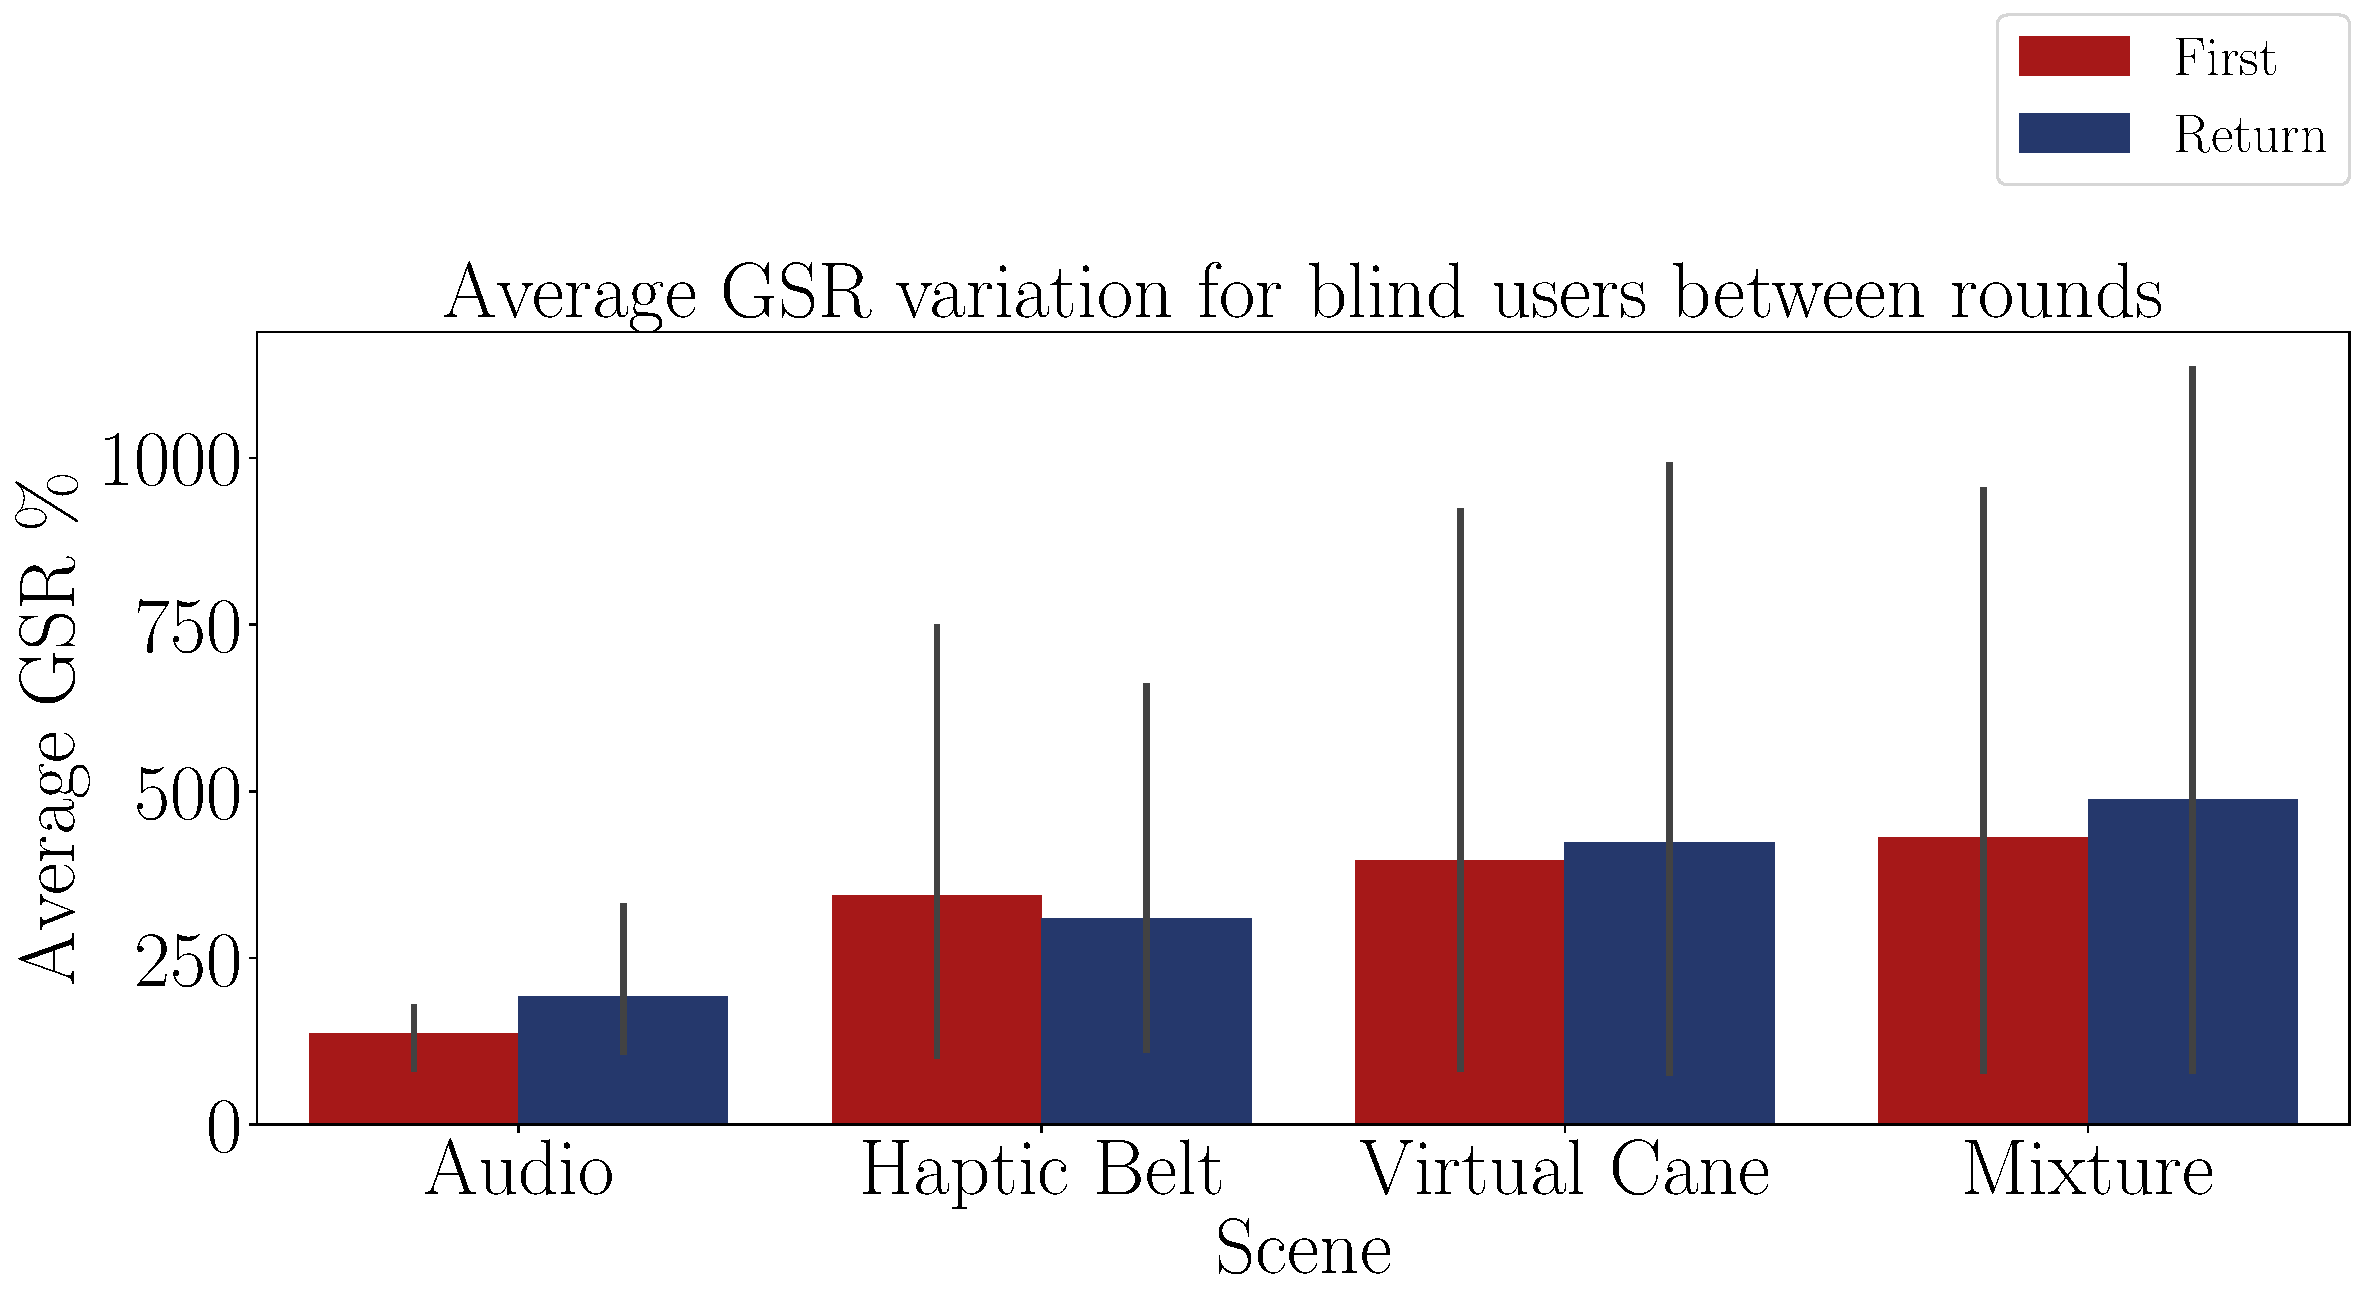
\includegraphics[width = 0.8\linewidth]{Resultados/GSR/Figuras/pdf/barplot_gsr_avg_4_scene_blind.pdf}
        \subcaption{Blind participants.}
        \label{fig:barplot_gsr_avg_4_scene_blind}
    \end{minipage}
    \begin{minipage}{\textwidth}
        \centering
        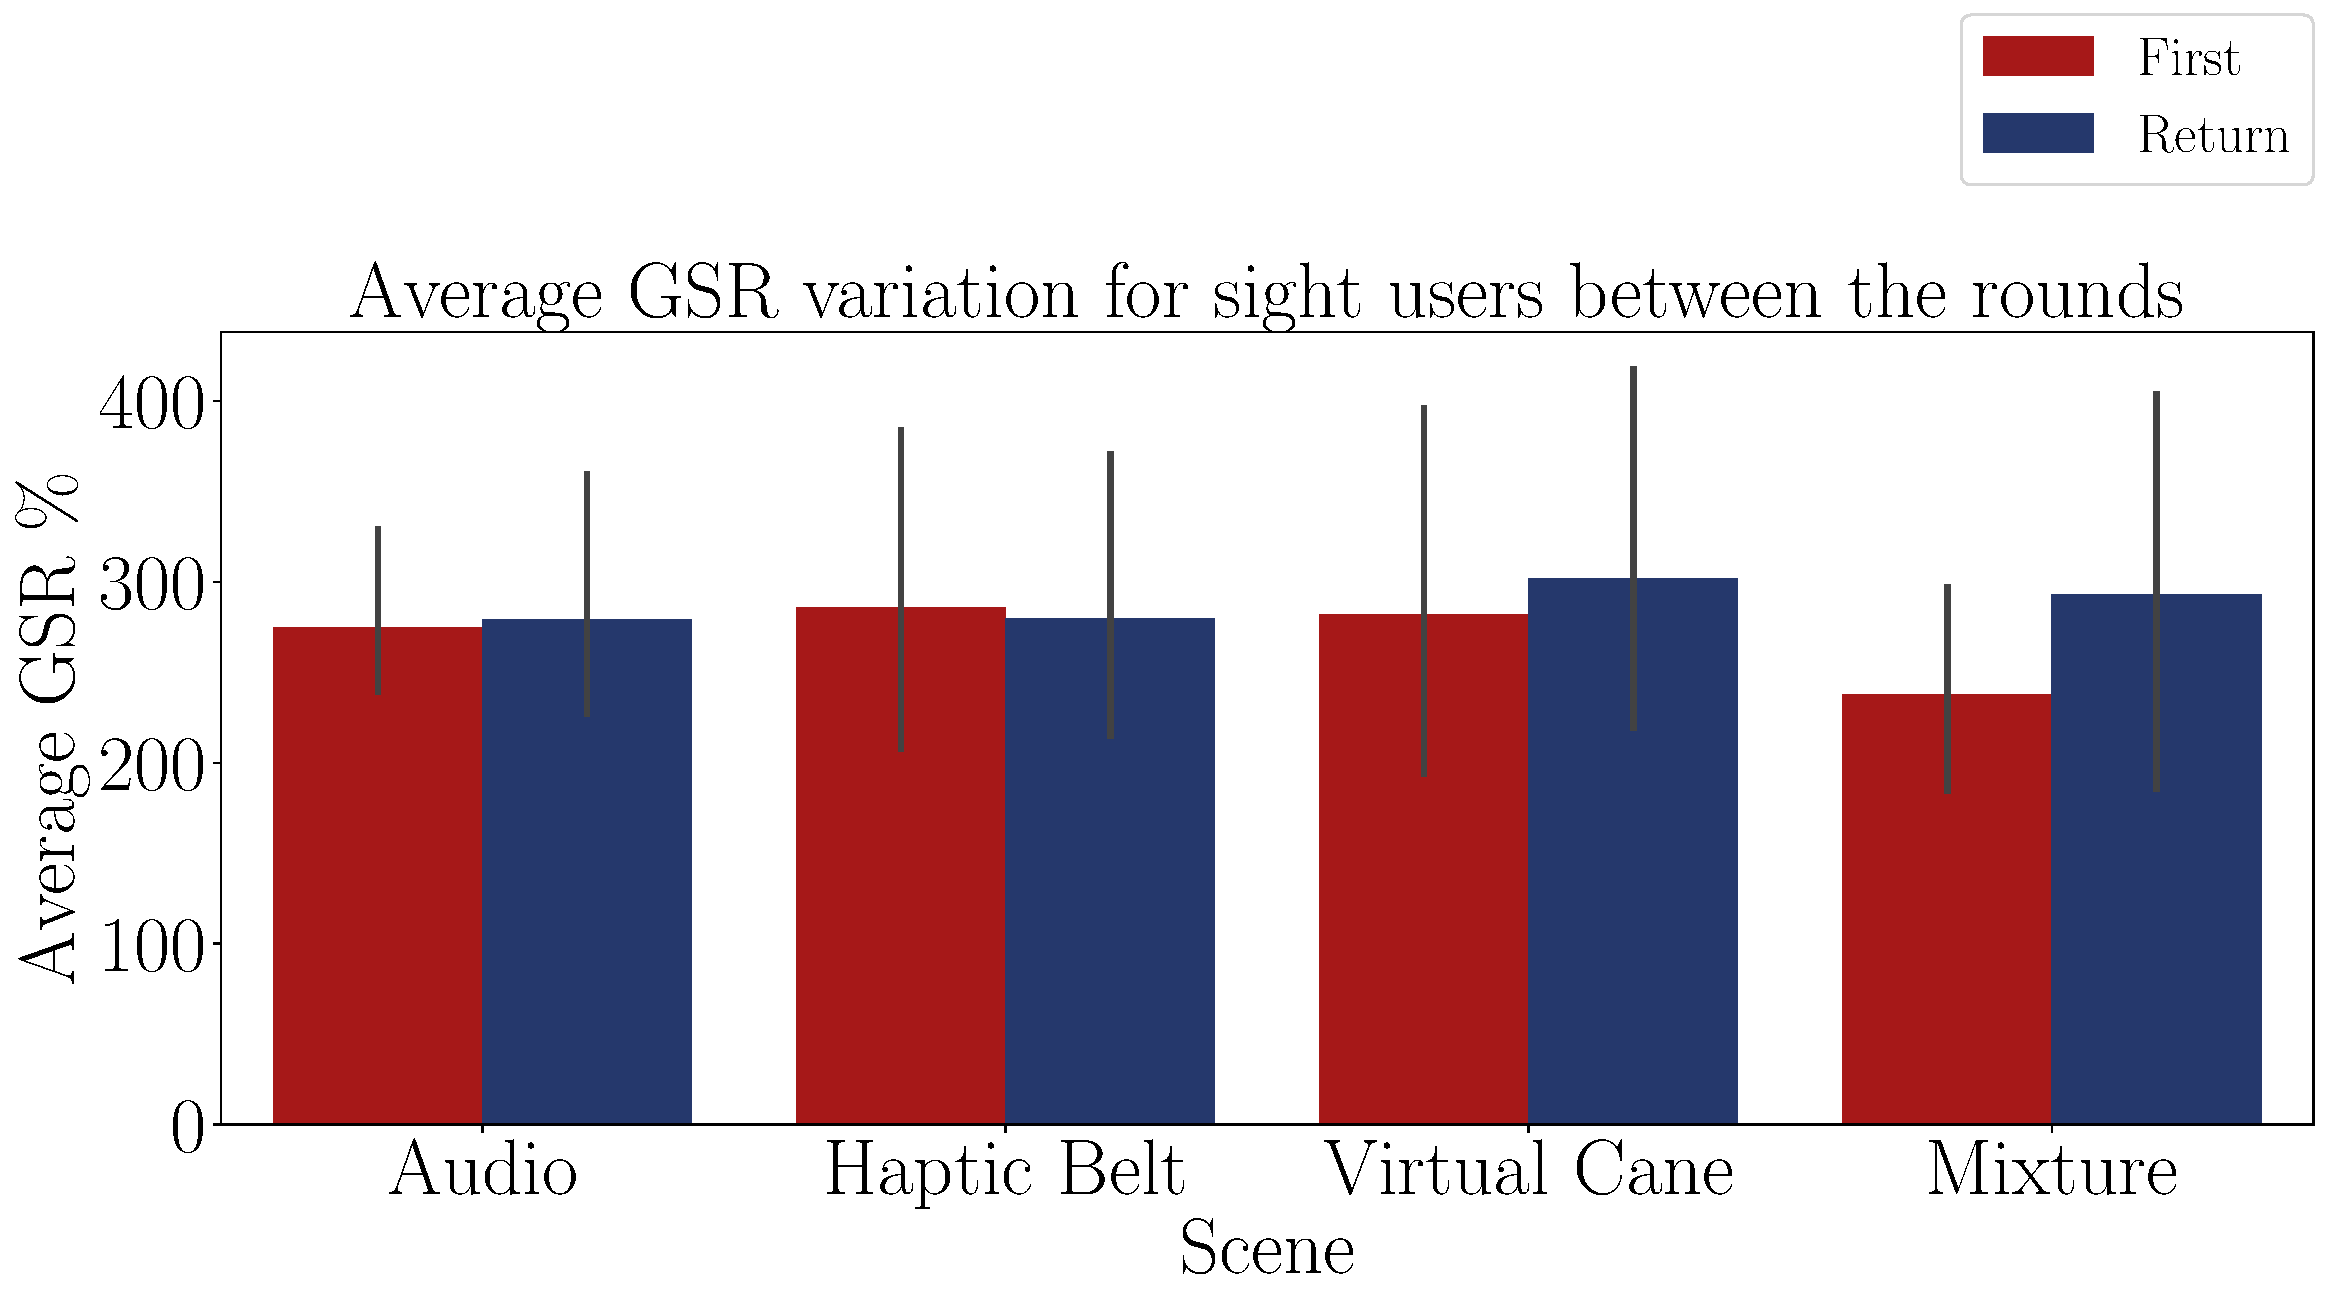
\includegraphics[width = 0.8\linewidth]{Resultados/GSR/Figuras/pdf/barplot_gsr_avg_4_scene_sight.pdf}
        \subcaption{Sight participants.}
        \label{fig:barplot_gsr_avg_4_scene_sight}
    \end{minipage}
    \caption{Barplot of the average GSR on each method and round.}
    \label{fig:barplot_gsr_avg_4_scene_blind_sight}
\end{figure}

\begin{figure}[!htb]
    \centering
    \begin{minipage}{0.45\textwidth}
        \centering
        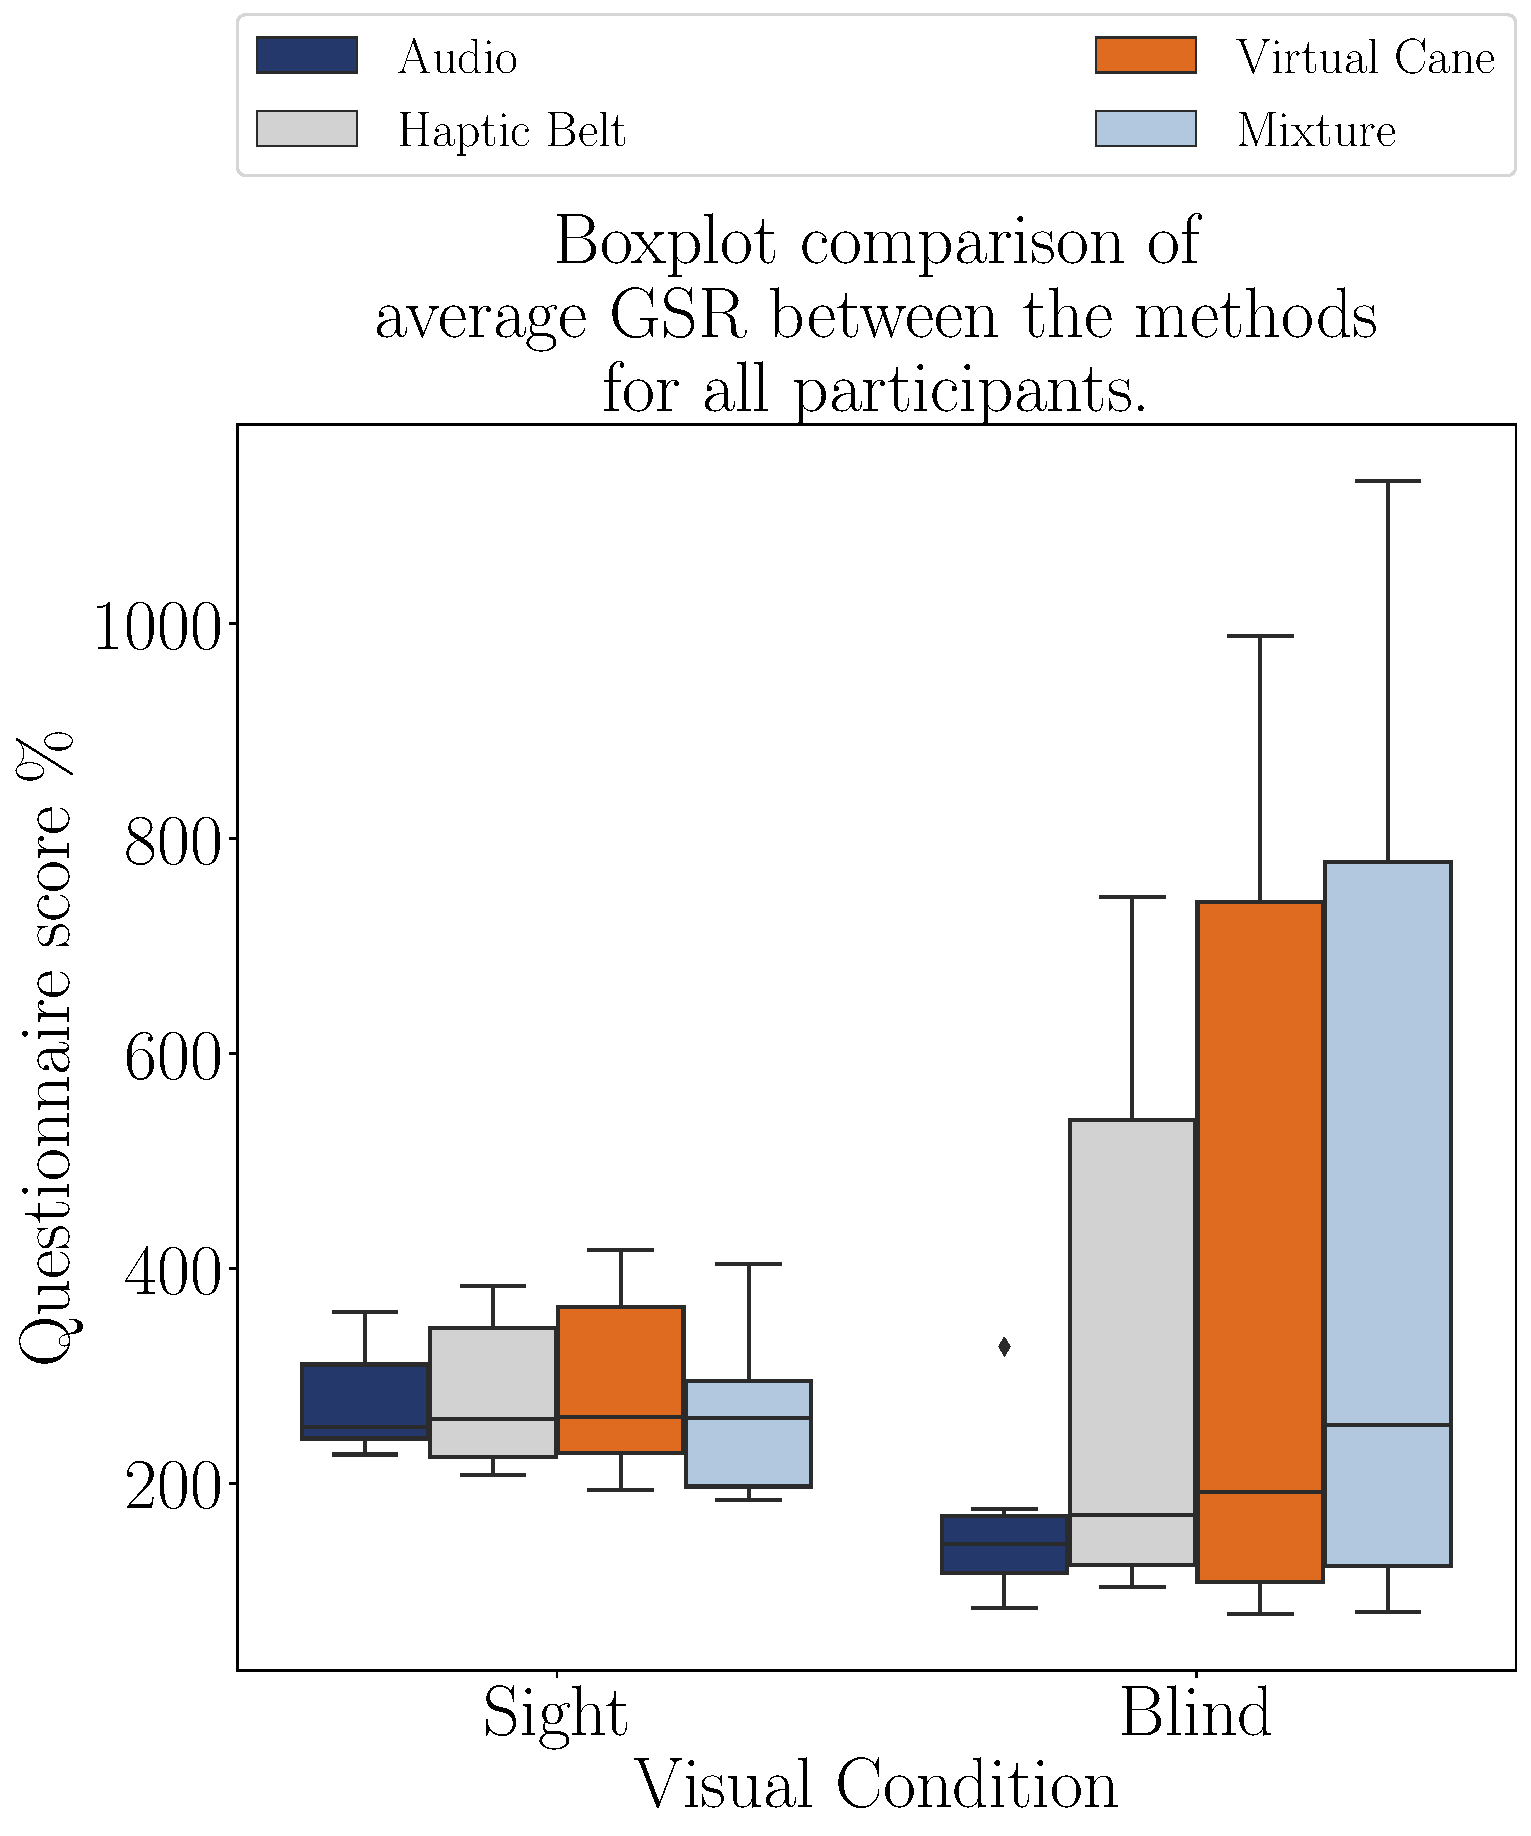
\includegraphics[width = 0.8\linewidth]{Resultados/GSR/Figuras/pdf/boxplot_gsr_avg_4_scene.pdf}
        \caption{Boxplot of the average GSR of the participants grouped by method.}
        \label{fig:boxplot_gsr_avg_4_scene}
    \end{minipage}
    \begin{minipage}{0.075\textwidth}
        \hfill
    \end{minipage}
    \begin{minipage}{0.45\textwidth}
        \centering
        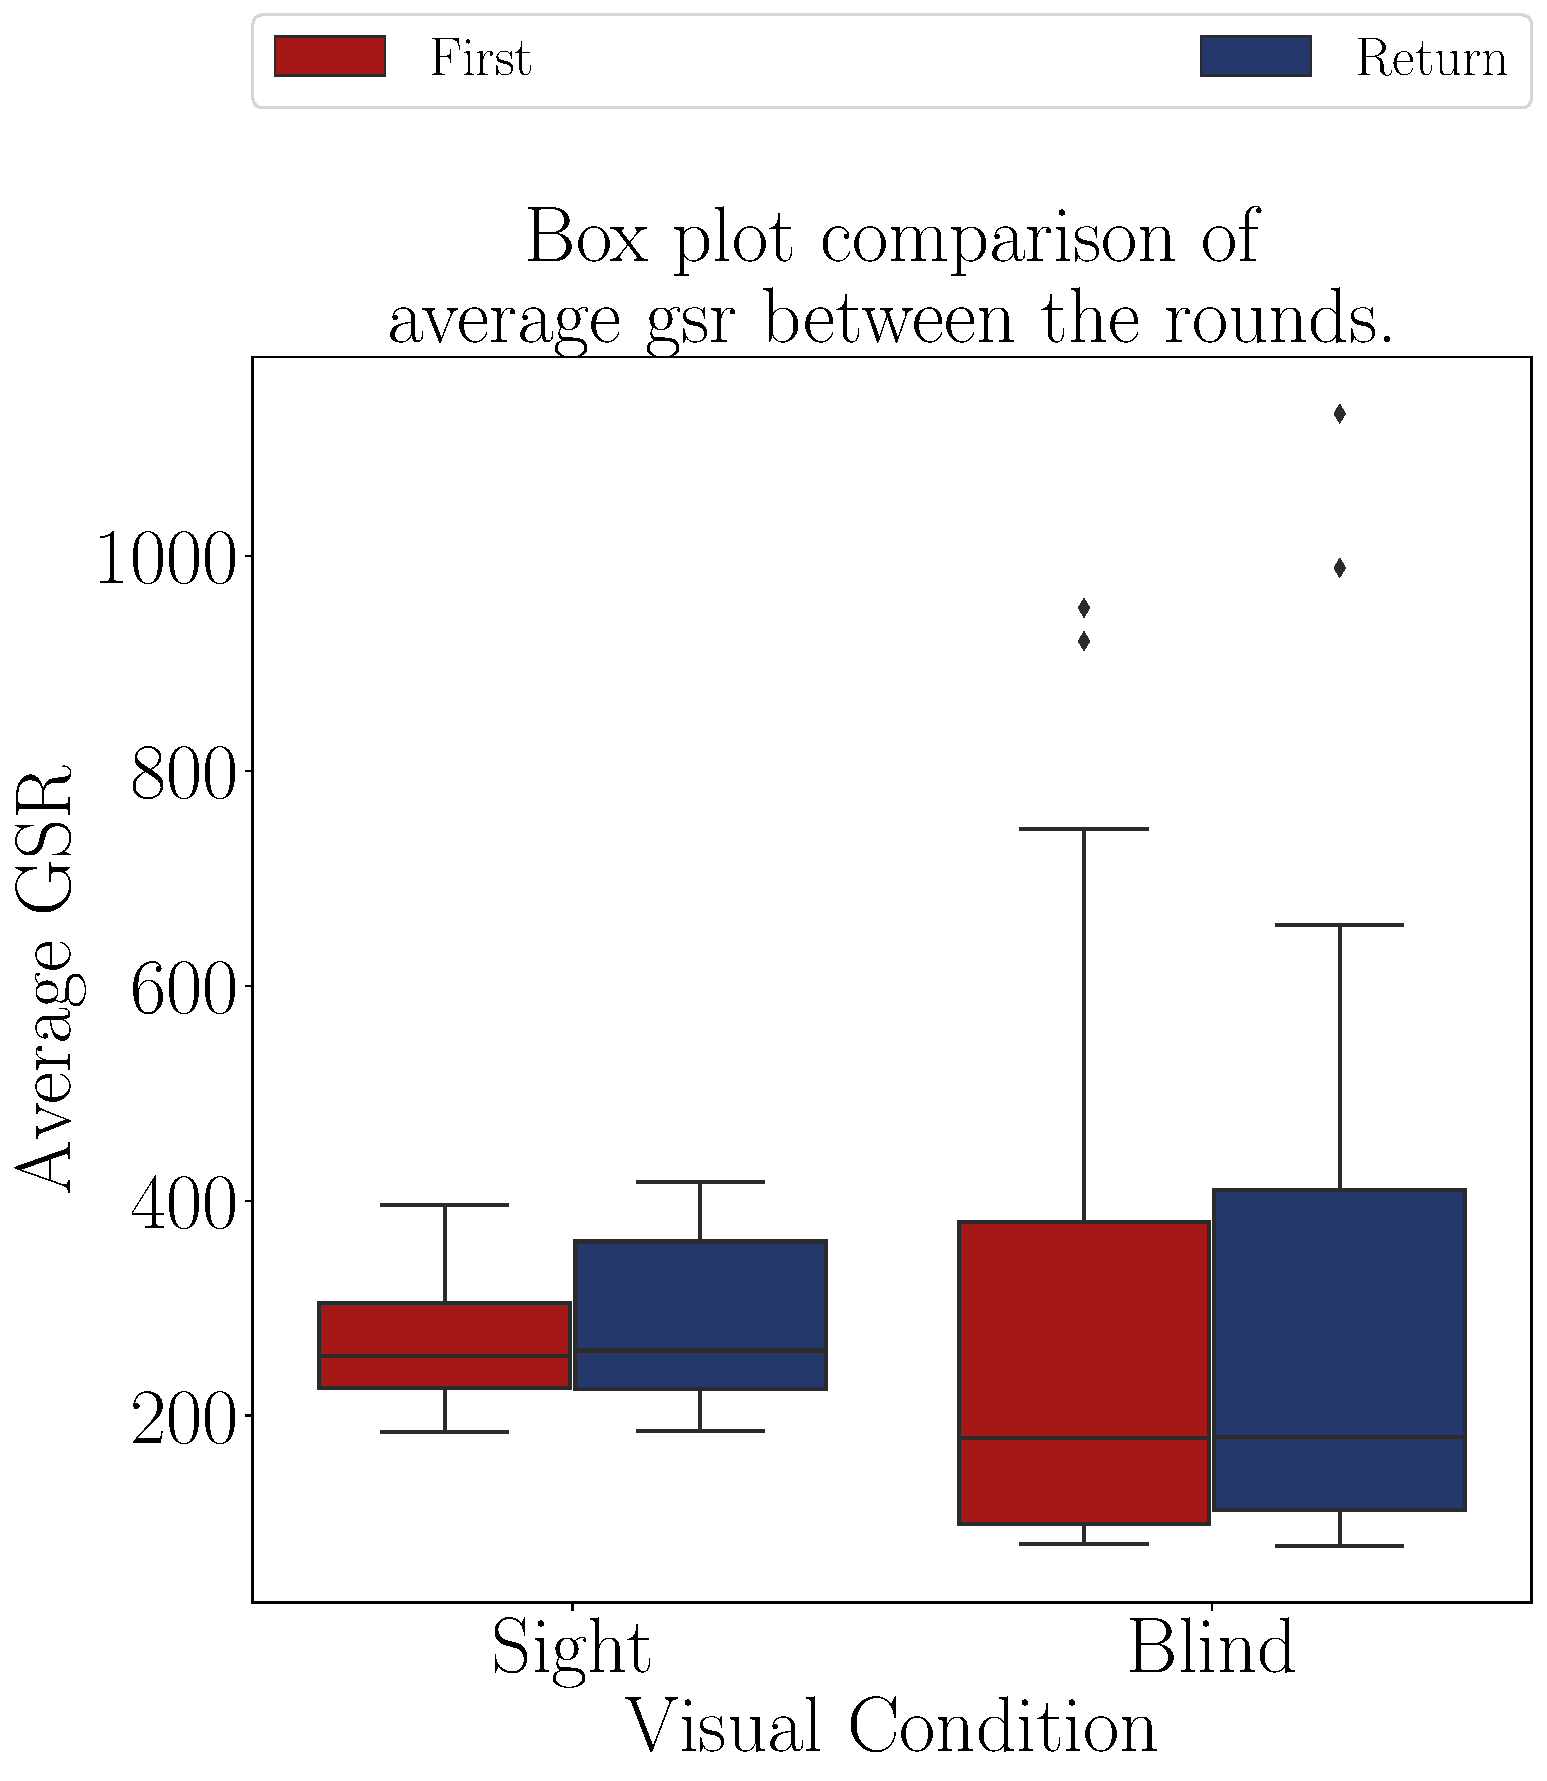
\includegraphics[width = 0.8\linewidth]{Resultados/GSR/Figuras/pdf/boxplot_gsr_avg_4_rounds.pdf}
        \caption{Boxplot of the average GSR of the participants grouped by round.}
        \label{fig:boxplot_gsr_avg_4_rounds}
    \end{minipage}
\end{figure}

Figures \ref{fig:qqplot_gsr_two_way_sight} and \ref{fig:residplot_gsr_two_way_sight} bring the QQ Plot and residual distribution. The results from ANOVA are presented in Table \ref{tab:blocanova_gsr_two_way_blind_sight}. In the case of blind participants, the p-value for the method is just slightly over the threshold, indicating a possible influence of the method. The same do not happen with sighted participants, where the p-value of the method factor is the highest one and well above the 0.05 threshold.
 
%The Table \ref{tab:gsr_average_group_noBase} shows the average skin conductance variation of both samples. It also shows that the presence of a haptic device increases the GSR, whilst the sight user had a basically constant GSR.
%
%
\begin{table}[!htb]
\centering
\caption{Average GSR variation grouped by participant and visual condition}
\label{tab:gsr_average_group_noBase}
\begin{tabular}{lrrrrr}
\toprule
{} &     Audio & \begin{tabular}[c]{@{}l@{}}Haptic\\ Belt\end{tabular} & \begin{tabular}[c]{@{}l@{}}Virtual\\ Cane\end{tabular} &   Mixture \\
Visual Condition &           &                                                       &                                                        &           \\
\midrule
Blind            &  164.10\% &                                              327.01\% &                                               409.57\% &  459.15\% \\
Sight            &  276.80\% &                                              282.80\% &                                               291.73\% &  265.50\% \\
\bottomrule
\end{tabular}
\end{table}



\begin{table}
    \caption{Anova p-value for the skin conductance average on each method}
    \label{tab:blocanova_gsr_two_way_blind_sight}
\begin{minipage}{0.45\textwidth}
    \subcaption{Blind participants}
    \input{Resultados/GSR/Tabelas/blocanova_gsr_two_way_blindsemBegin.tex}
\end{minipage}
\begin{minipage}{0.45\textwidth}
    \subcaption{Sight participants}
    \input{Resultados/GSR/Tabelas/blocanova_gsr_two_way_sightsemBegin.tex}
\end{minipage}
\end{table}

\begin{figure}[!htb]
    \centering
    %\vspace{-15.0cm}
    \begin{minipage}{0.45\textwidth}
        \centering
        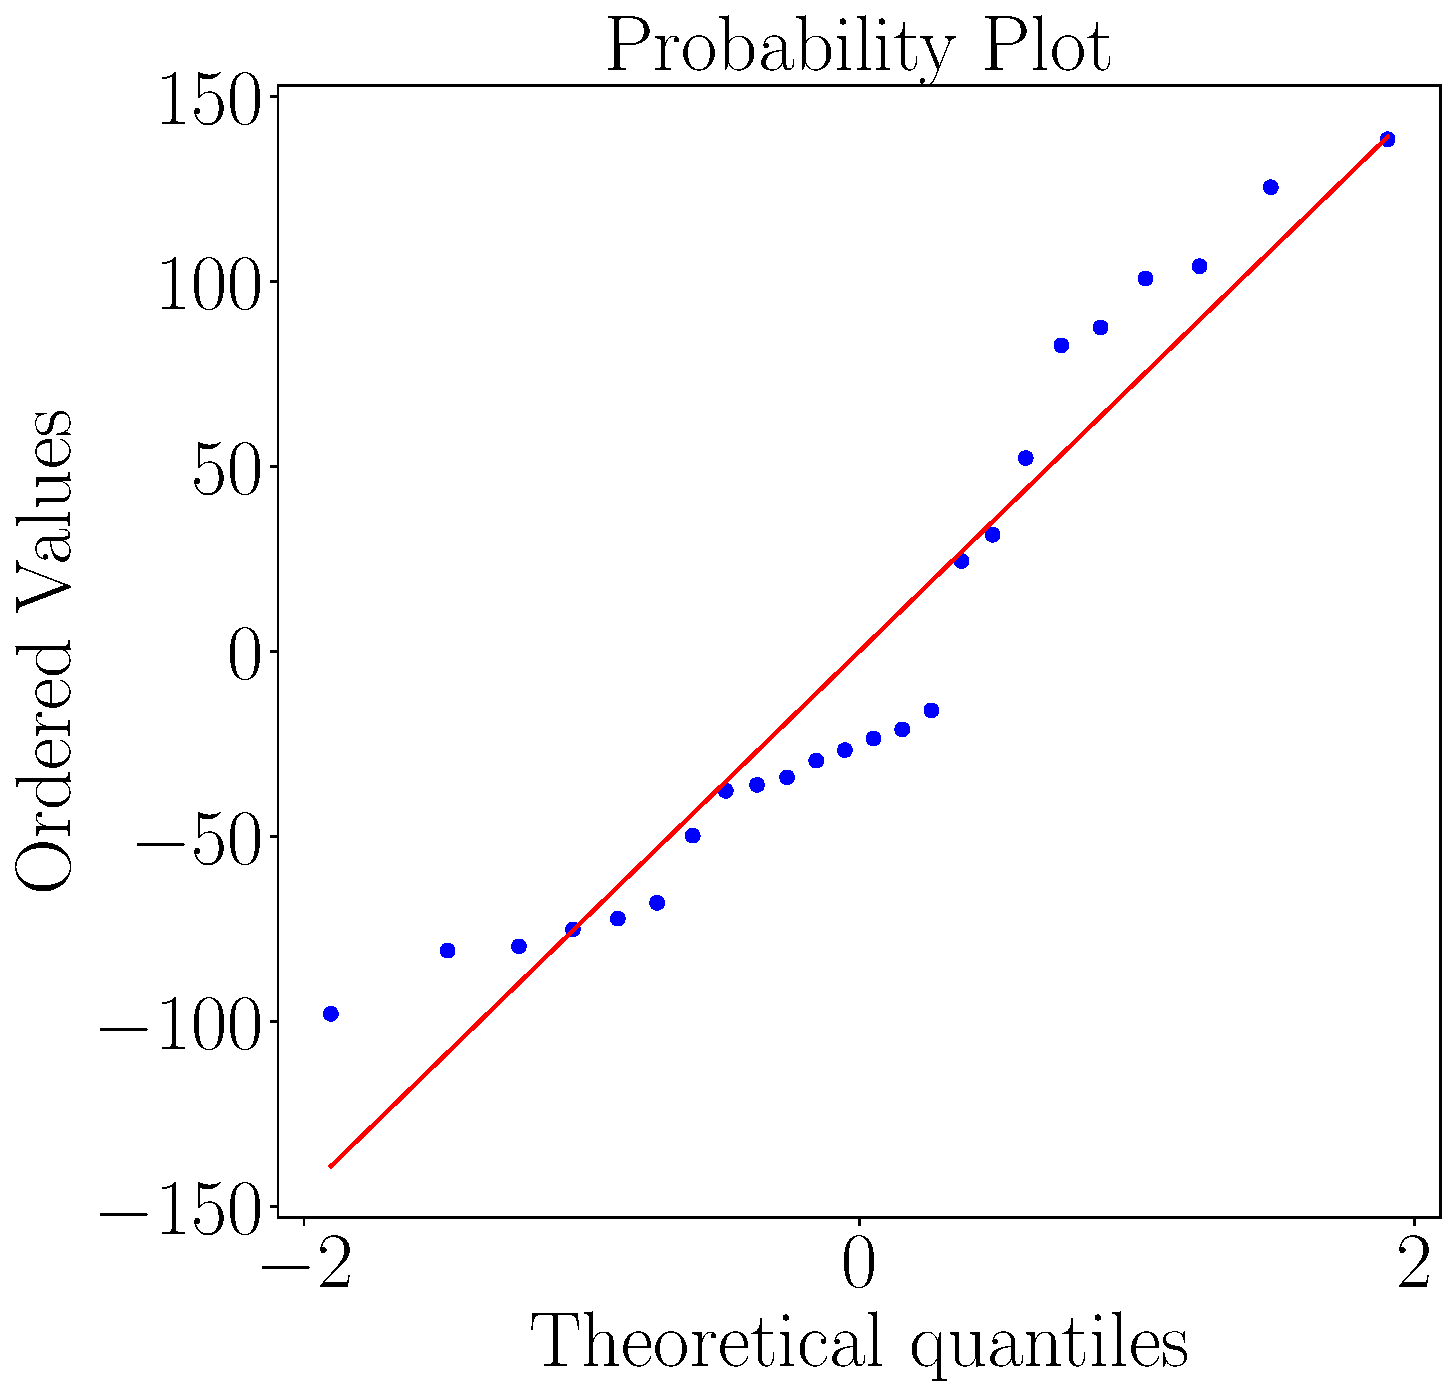
\includegraphics[width = 0.8\linewidth]{Resultados/GSR/Figuras/pdf/qqplot_gsr_two_way_sight.pdf}
        \caption{QQ plot of the average skin conductance of the sight participants on each method.}
        \label{fig:qqplot_gsr_two_way_sight}
    \end{minipage}
    \begin{minipage}{0.075\textwidth}
        \hfill
    \end{minipage}
    \begin{minipage}{0.45\textwidth}
        \centering
        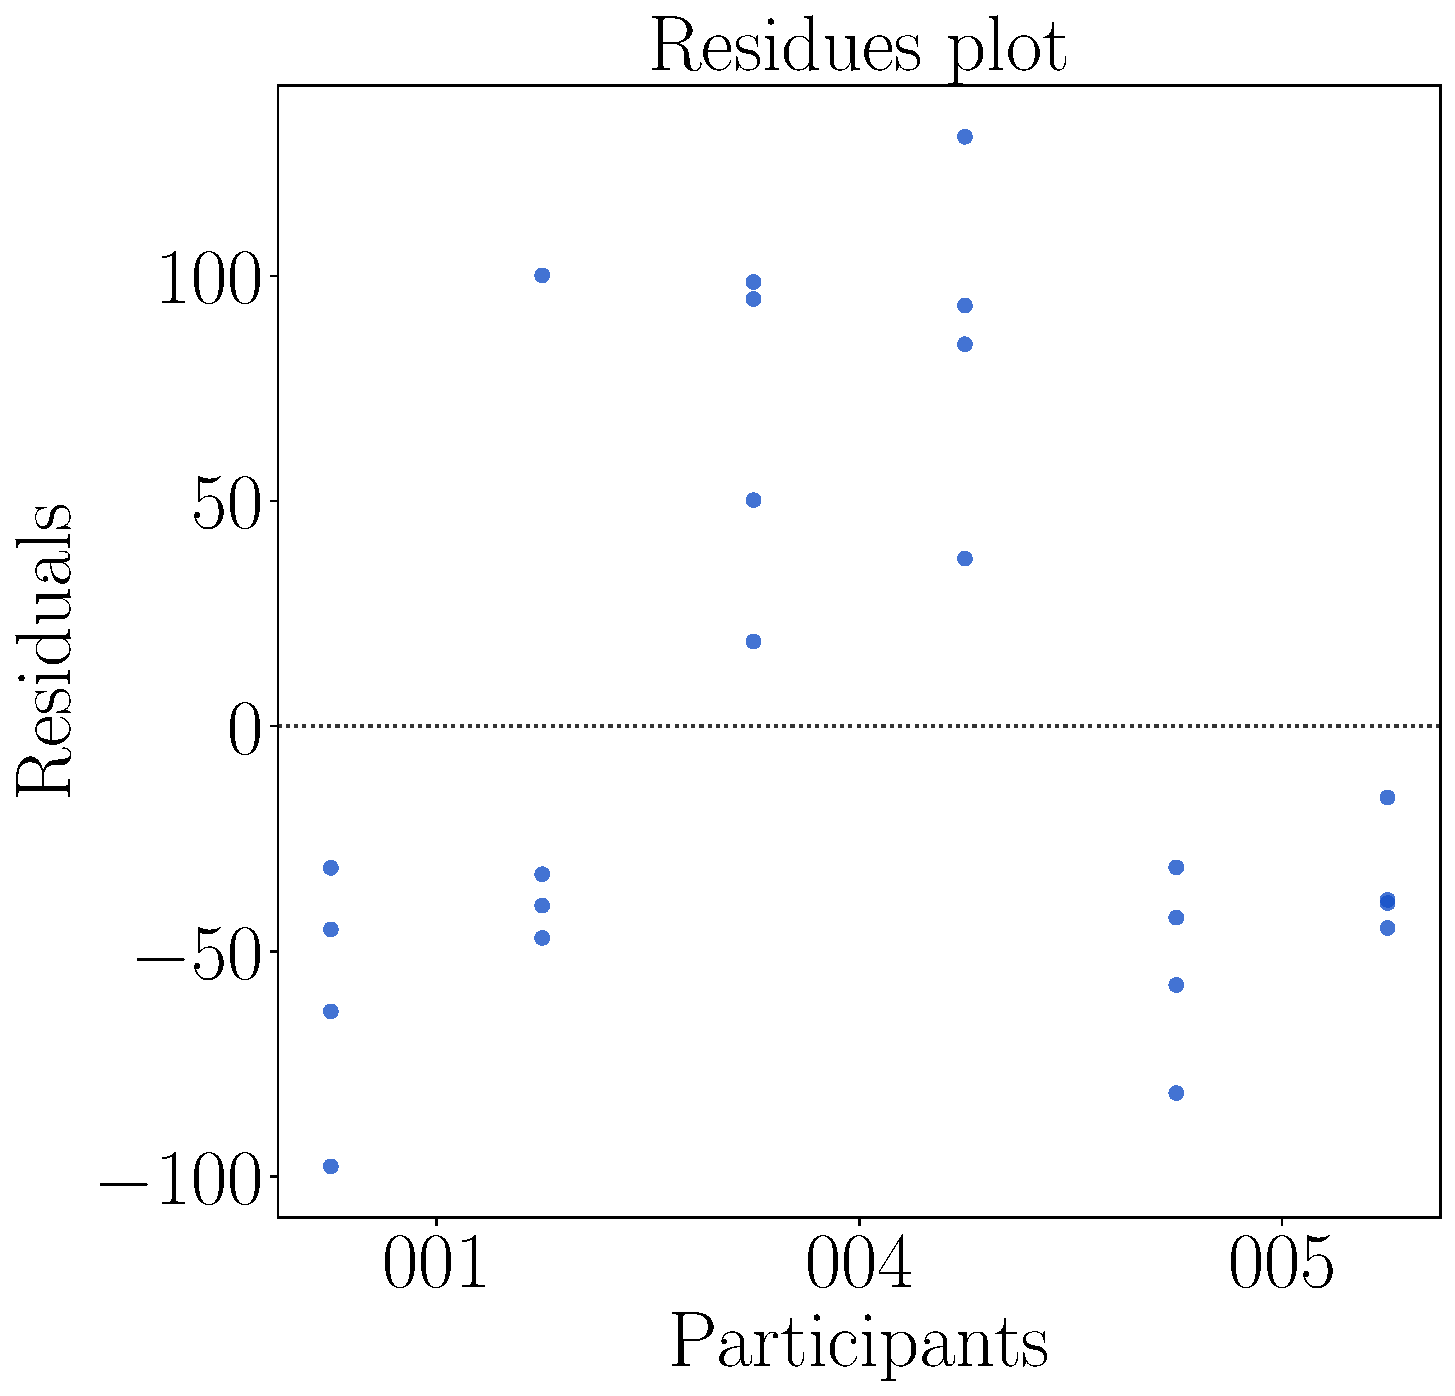
\includegraphics[width = 0.8\linewidth]{Resultados/GSR/Figuras/pdf/residplot_gsr_two_way_sight.pdf}
        \caption{Residual plot of the average skin conductance score the sight participants on each method.}
        \label{fig:residplot_gsr_two_way_sight}
    \end{minipage}
\end{figure}

\FloatBarrier